%%%%%%%%%%%%%%%%%%%%%%%%%%%%%%%%%%%%%%%%%%%%%%%%%%%%%%%%%%%%%%%%%%%%% 
%% This is a (brief) model paper using the achemso class 
%% The document class accepts keyval options, which should include 
%% the target journal and optionally the manuscript type. 
%%%%%%%%%%%%%%%%%%%%%%%%%%%%%%%%%%%%%%%%%%%%%%%%%%%%%%%%%%%%%%%%%%%%% 
\documentclass[journal=jpcbfk,manuscript=article]{achemso} 
 
%%%%%%%%%%%%%%%%%%%%%%%%%%%%%%%%%%%%%%%%%%%%%%%%%%%%%%%%%%%%%%%%%%%%% 
%% Place any additional packages needed here.  Only include packages 
%% which are essential, to avoid problems later. Do NOT use any 
%% packages which require e-TeX (for example etoolbox): the e-TeX 
%% extensions are not currently available on the ACS conversion 
%% servers. 
%%%%%%%%%%%%%%%%%%%%%%%%%%%%%%%%%%%%%%%%%%%%%%%%%%%%%%%%%%%%%%%%%%%%% 

%% Workaround for malfunctioning textsuperscript with pdfx and T1 encoding
\let\tmpa\textsuperscript
\DeclareTextCommandDefault{\textsuperscript}{\tmpa}

\usepackage[x11names]{xcolor}  % typesetting in color
%% Generate PDF/A-2u
\usepackage[a-2u]{pdfx}
 
\usepackage[super]{natbib}         % citation style AUTHOR (YEAR), or AUTHOR [NUMBER]

\usepackage{achemso}  
\usepackage{rotating}  
%\usepackage{times} 
%\usepackage{lmodern}    %% Prefer Latin Modern fonts
\usepackage{graphicx} 
\usepackage{setspace} 
\usepackage{amsmath} 
\usepackage{epstopdf} 
\usepackage{csquotes} 
\usepackage{mhchem} 
\usepackage{chemfig} 
\usepackage[obeyFinal]{easy-todo}
\usepackage[english]{babel}
 
\usepackage{subfig}
\usepackage{dcolumn}        % improved alignment of table columns
\usepackage{booktabs}       % improved horizontal lines in tables
\usepackage{paralist}       % improved enumerate and itemize

%% Character encoding: usually latin2, cp1250 or utf8:
\usepackage[utf8]{inputenc}
\usepackage[T1]{fontenc}

%\usepackage{markdown}  
 
%% The hyperref package for clickable links in PDF and also for storing
%% metadata to PDF (including the table of contents).
%% Most settings are pre-set by the pdfx package.
\hypersetup{unicode}
\hypersetup{breaklinks=true}
\hypersetup{colorlinks,allcolors=DodgerBlue4}
 
%%%%%%%%%%%%%%%%%%%%%%%%%%%%%%%%%%%%%%%%%%%%%%%%%%%%%%%%%%%%%%%%%%%%% 
%% If issues arise when submitting your manuscript, you may want to 
%% un-comment the next line.  This provides information on the 
%% version of every file you have used. 
%%%%%%%%%%%%%%%%%%%%%%%%%%%%%%%%%%%%%%%%%%%%%%%%%%%%%%%%%%%%%%%%%%%%% 
%%\listfiles 
 
%%%%%%%%%%%%%%%%%%%%%%%%%%%%%%%%%%%%%%%%%%%%%%%%%%%%%%%%%%%%%%%%%%%%% 
%% Place any additional macros here.  Please use \newcommand* where 
%% possible, and avoid layout-changing macros (which are not used 
%% when typesetting). 
%%%%%%%%%%%%%%%%%%%%%%%%%%%%%%%%%%%%%%%%%%%%%%%%%%%%%%%%%%%%%%%%%%%%% 
\newcommand*\mycommand[1]{\texttt{\emph{#1}}} 
%%% Custom variables
% width suitable for fitting into a column in 1-column page layout
\newlength{\figwidth}
\setlength{\figwidth}{9 cm} 
\newlength{\figwidthsmall}
\setlength{\figwidthsmall}{6 cm} 
\newlength{\figwidthfull}
\setlength{\figwidthfull}{14 cm} 
\newlength{\figheightsmall}
\setlength{\figheightsmall}{8 cm} 
\newlength{\figheight}
\setlength{\figheight}{12 cm} 

 
%%%%%%%%%%%%%%%%%%%%%%%%%%%%%%%%%%%%%%%%%%%%%%%%%%%%%%%%%%%%%%%%%%%%% 
%% Meta-data block 
%% --------------- 
%% Each author should be given as a separate \author command. 
%% 
%% Corresponding authors should have an e-mail given after the author 
%% name as an \email command. Phone and fax numbers can be given 
%% using \phone and \fax, respectively; this information is optional. 
%% 
%% The affiliation of authors is given after the authors; each 
%% \affiliation command applies to all preceding authors not already 
%% assigned an affiliation. 
%% 
%% The affiliation takes an option argument for the short name.  This 
%% will typically be something like "University of Somewhere". 
%% 
%% The \altaffiliation macro should be used for new address, etc. 
%% On the other hand, \alsoaffiliation is used on a per author basis 
%% when authors are associated with multiple institutions. 
%%%%%%%%%%%%%%%%%%%%%%%%%%%%%%%%%%%%%%%%%%%%%%%%%%%%%%%%%%%%%%%%%%%%% 
 
\author{Josef Melcr} 
\email{melcr@uochb.cas.cz} 
%%\homepage[]{https://jmelcr.github.io/}
\affiliation{Institute of Organic Chemistry and Biochemistry, 
Academy of Sciences of the Czech Republic,  
Prague 6, Czech Republic} 
\author{Pavel Jungwirth} 
%%\homepage[]{http://jungwirth.uochb.cas.cz/}
\affiliation{Institute of Organic Chemistry and Biochemistry, 
Academy of Sciences of the Czech Republic,  
Prague 6, Czech Republic} 
\alsoaffiliation{Department of Physics, Tampere University of Technology, P.O. Box 692, FI-33101 
Tampere, Finland} 
%SAMULI: We need to put tiago because the experimental acyl chain order parameters
\author{Tiago Ferreira}
\affiliation{Halle} 
\author{O. H. Samuli Ollila} 
\email{samuli.ollila@helsinki.fi} 
%%\homepage[]{Your web page} 
\affiliation{Institute of Organic Chemistry and Biochemistry, 
Academy of Sciences of the Czech Republic,  
Prague 6, Czech Republic} 
\alsoaffiliation{Institute of Biotechnology, University of Helsinki} 
 
 
%\author{Andrew N. Other} 
%\altaffiliation{A shared footnote} 
%\author{Fred T. Secondauthor} 
%\altaffiliation{Current address: Some other place, Othert\"own, 
%Germany} 
%\author{I. Ken Groupleader} 
%\altaffiliation{A shared footnote} 
%\email{i.k.groupleader@unknown.uu} 
%\phone{+123 (0)123 4445556} 
%\fax{+123 (0)123 4445557} 
%\affiliation[Unknown University] 
%{Department of Chemistry, Unknown University, Unknown Town} 
%\alsoaffiliation[Second University] 
%{Department of Chemistry, Second University, Nearby Town} 
%\author{Susanne K. Laborator} 
%\email{s.k.laborator@bigpharma.co} 
%\affiliation[BigPharma] 
%{Lead Discovery, BigPharma, Big Town, USA} 
%\author{Kay T. Finally} 
%\affiliation[Unknown University] 
%{Department of Chemistry, Unknown University, Unknown Town} 
%\alsoaffiliation[Second University] 
%{Department of Chemistry, Second University, Nearby Town} 
 
%%%%%%%%%%%%%%%%%%%%%%%%%%%%%%%%%%%%%%%%%%%%%%%%%%%%%%%%%%%%%%%%%%%%% 
%% The document title should be given as usual. Some journals require 
%% a running title from the author: this should be supplied as an 
%% optional argument to \title. 
%%%%%%%%%%%%%%%%%%%%%%%%%%%%%%%%%%%%%%%%%%%%%%%%%%%%%%%%%%%%%%%%%%%%% 
%\title[] 
%  {Accurate interactions of cations with 
%   neutral and negatively charged membranes 
%   via combination of experiments and molecular simulation}

%%SAMULI: new suggestion for the preliminary title
\title[] 
  {Effective Inclusion of Electronic Polarization to a Negatively Charged Membrane}

%%%%%%%%%%%%%%%%%%%%%%%%%%%%%%%%%%%%%%%%%%%%%%%%%%%%%%%%%%%%%%%%%%%%% 
%% Some journals require a list of abbreviations or keywords to be 
%% supplied. These should be set up here, and will be printed after 
%% the title and author information, if needed. 
%%%%%%%%%%%%%%%%%%%%%%%%%%%%%%%%%%%%%%%%%%%%%%%%%%%%%%%%%%%%%%%%%%%%% 
\abbreviations{IR,NMR,UV,MD,ECC,PC,PS,POPS,POPS} 
\keywords{MD simulation, molecular modeling, 
          polarizability, polarization,
          phospholipids, phosphatidylserine} 

%%%%%%%%%%%%%%%%%%%%%%%%%%%%%%%%%%%%%%%%%%%%%%%%%%%%%%%%%%%%%%%%%%%%% 
%% The manuscript does not need to include \maketitle, which is 
%% executed automatically. 
%%%%%%%%%%%%%%%%%%%%%%%%%%%%%%%%%%%%%%%%%%%%%%%%%%%%%%%%%%%%%%%%%%%%% 
\begin{document} 
 
%%%%%%%%%%%%%%%%%%%%%%%%%%%%%%%%%%%%%%%%%%%%%%%%%%%%%%%%%%%%%%%%%%%%% 
%% The "tocentry" environment can be used to create an entry for the 
%% graphical table of contents. It is given here as some journals 
%% require that it is printed as part of the abstract page. It will 
%% be automatically moved as appropriate. 
%%%%%%%%%%%%%%%%%%%%%%%%%%%%%%%%%%%%%%%%%%%%%%%%%%%%%%%%%%%%%%%%%%%%% 
\begin{tocentry} 
 
Some journals require a graphical entry for the Table of Contents. 
This should be laid out ``print ready'' so that the sizing of the 
text is correct. 
 
Inside the \texttt{tocentry} environment, the font used is Helvetica 
8\,pt, as required by \emph{Journal of the American Chemical 
Society}. 
 
The surrounding frame is 9\,cm by 3.5\,cm, which is the maximum 
permitted for  \emph{Journal of the American Chemical Society} 
graphical table of content entries. The box will not resize if the 
content is too big: instead it will overflow the edge of the box. 
 
This box and the associated title will always be printed on a 
separate page at the end of the document. 
 
\end{tocentry} 
 
%%%%%%%%%%%%%%%%%%%%%%%%%%%%%%%%%%%%%%%%%%%%%%%%%%%%%%%%%%%%%%%%%%%%% 
%% The abstract environment will automatically gobble the contents 
%% if an abstract is not used by the target journal. 
%%%%%%%%%%%%%%%%%%%%%%%%%%%%%%%%%%%%%%%%%%%%%%%%%%%%%%%%%%%%%%%%%%%%% 
 
 
 
\begin{abstract} 

\textbf{Main message: 
ECC generally improves interaction and structure of both neutral and charged molecules. 
Polarizability is necessarry for accurate simulations of cellular membranes at physiological ionic conditions.} 

%%% SAMULI: I commented this out because it way too general. We can write abstract later when the final content is clear.

%Binding affinities and stoichiometries of sodium and calcium ions to phospholipid bilayers are of paramount significance in the properties and functionality of cellular membranes. Current estimates of binding affinities and stoichiometries of cations are, however, controversial due to limitations in the available experimental and theoretical methods. Experimentally one can assess these parameters by titrating several membrane properties as a function of the ion concentration. However, the interpretation of the experiments relies on theoretical models, as direct molecular information is not available. 

%Classical molecular dynamics (MD) simulations provide details of the ion binding process with atomistic resolution, therefore offering all the necessary information to interpret experimental data without the need to resort to over-simplified models. However, the accuracy of the currently available lipid models when interacting with ions is not sufficient for such interpretation \cite{catte16}. Recently, we have improved the binding details of sodium and calcium ions to the 1-Palmitoyl-2-oleoyl-phosphatidylcholine (POPC) bilayer by implicitly including electronic polarization as a mean field correction, known as the electronic continuum correction (ECC). Our improved ECC-POPC model reproduces not only the experimentally measured structural parameters for the ion-free membrane, but also improves significantly the response of lipid head group to a bound positive charge, and the binding affinities of sodium and calcium ions. \cite{melcr18}

%We are now extending our work to other lipid membranes composed of larger varieties of different biologically relevant lipids. In particular, we focus our attention on membranes with 
%	%phosphatidylethanolamine (PE) and 
%	negatively charged phosphatidylserine (PS) lipids. 
%	We compare available NMR and x-ray experiments with MD simulations to obtain atomistic-resolution picture of the interactions between cations and phospholipid membranes. Our results indicate that electronic polarization is a non-negligable interaction, which dramatically improves the description of cation binding to phospholipid membranes. 
\end{abstract} 
 
 
%\begin{abstract} 
%  This is an example document for the \textsf{achemso} document 
%  class, intended for submissions to the American Chemical Society 
%  for publication. The class is based on the standard \LaTeXe\ 
%  \textsf{report} file, and does not seek to reproduce the appearance 
%  of a published paper. 
 
%  This is an abstract for the \textsf{achemso} document class 
%  demonstration document.  An abstract is only allowed for certain 
%  manuscript types.  The selection of \texttt{journal} and 
%  \texttt{manuscript} will determine if an abstract is valid.  If 
%  not, the class will issue an appropriate error. 
%\end{abstract} 
 
%%%%%%%%%%%%%%%%%%%%%%%%%%%%%%%%%%%%%%%%%%%%%%%%%%%%%%%%%%%%%%%%%%%%% 
%% Start the main part of the manuscript here. 
%%%%%%%%%%%%%%%%%%%%%%%%%%%%%%%%%%%%%%%%%%%%%%%%%%%%%%%%%%%%%%%%%%%%% 
 
 
 
\section{Introduction} 

Lipids with negatively charged headgroups, like phophatidylserine
play important role in biomembranes. 
Signaling molecules in cells interact with lipid membranes 
due to specific, often electrostatically driven, interactions 
with anionic lipids \cite{lemmon08,leventis10}.
Anionic lipids and their interactions with ions play also role in membrane
fusion \cite{??}. \todo{Pavel can probably improve this and give a citation}
These interactions depend both on
the chemical details of lipid headgroups as well as 
on the binding of counter and co-ions to anionic membranes. 

Various interaction schemes have been proposed for the negatively charged
lipids with ions and other lipids. 
Some studies suggest that the
binding constant of ions to negatively charged lipids is similar to that of zwitterionic lipids,
and the binding affinity is increased only due to the increased cation
concentration in the vicinity of the membrane \cite{seelig90,sinn06}.
On the other hand, calcium forms dehydrated complexes with PS headgroups
which cause phase separation \cite{hauser77,kurland79,hauser85,feigenson86,mattai89,roux90,roux91,boettcher11}.
Different theories are difficult to evaluate experimentally,
especially with physiological ion concentrations which are typically quite low.

Spectroscopic experiments give detailed information about the
interactions between ions and PS lipids, but the data is often indirect and difficult to
interpret \cite{hauser77,kurland79,eisenberg79,hauser83,dluhy83,hauser85,feigenson86,mattai89,roux90,roux91,boettcher11}.
Classical molecular dynamics (MD) simulations give
access to all the details, but the current non-polarizable force fields are not
sufficiently accurate to interpret the interactions between anionic
lipid headgroups and other lipids or ions \cite{NMRlipidsIV}.
%%%%%%%%%%%%%%%%%%%%%%%%%%%%%%%%
%% On the simulation part .. %%%
%%%%%%%%%%%%%%%%%%%%%%%%%%%%%%%%
%From the perspective of phospholipid bilayers,
There are force field parameters for neutral lipids PC and PE 
with explicit polarizability using the Classical Durde model. \cite{chowdhary13, chowdhary17}
While such a model shows a potential improvement over non-polarizable force fields from many perspectives -- 
for example accounting for polarizability has a significant impact on the dipole potential of a membrane \cite{harder2009} -- 
the non-polarizable version of the same force field 
performes comparably well at a fraction of the computational cost 
of the models with explicit polarization. \citep{lucas12,chowdhary13} 

Short paragraph describing previous MD-work on this topic (PS), i.e., \dots 
\todo{SAMULI: Controversies in previous simulations (https://doi.org/10.1016/j.bpj.2018.08.044 and
  Melcrova et al. Scientific Reports | 6:38035 | DOI: 10.1038/srep38035) should be mentioned also
in the intro.}

An empirical scaling factor, which reduces electrostatic forces between molecules, 
is a well known concept in molecular modelling;
such an approach was adopted in the early simulations of lipid bilayers \cite{egberts94, berendsen1996},
in force fields employing explicit polarization \cite{lemkul2016empirical},
or in the simulations of ionic liquids \cite{Bhargava2007}. 
%An improvement of permeability of charged solutes in the gramicidin A channel 
%is observed with a force field using charge equilibration to model polarizability. \cite{lucas2012} 
At the same time, 
the implicit inclusion of electronic polarizability to lipid models
via charge re-scaling using electronic continuum correction (ECC) 
substantially improved the interactions between cations and zwitterionic lipids \cite{melcr18}. 


Here, we extend the approach to anionic PS lipids.
The newly developed model termed ECC-POPS 
not only describes the interactions of PS with ions more accurately, 
but also improves the structure of the PS head group 
and its interactions with PC in mixed lipid bilayers. 
The results pave the way to more realistic MD simulations 
of both neutral and negatively charged lipid bilayers 
for a wide range of applications.


 
\section{Methods} 
 
\subsection{Electronic continuum correction for PS lipids}\label{section:ecc} 

\todo{Joe: this paragraph requires editing.}
The lack of electronic polarizability has been a concern since the
early days of classical MD simulations of lipids \cite{jonsson86,egberts94, berendsen1996},
where the atomic charges were scaled by a factor of 1/2 to effectively
include the electrostatic screening from the missing electronic polarizability.
The electronic continuum correction (ECC) is a more sophisticated version of the charge scaling.

The polarization of electrons in ECC-lipids uses the implicit method termed electronic continuum correction (ECC). \cite{leontyev09, Pluharova2014, martinek17, melcr18} 
In this method, a system of polarizable particles is represented 
with an equivalent system of particles with fixed charges,
which account for the electronic polarizability \emph{implicitly}. 
This is practically achieved by rescaling the charges with a pre-determined scaling factor, $f_q$,
which is derived from the high-frequency dielectric constant of electrons, $\epsilon_{el}$, as
\begin{equation}
  f_q = \frac{1}{\sqrt{\epsilon_{el}}} ,
\end{equation}
The value of $\epsilon_{el} = 1.78$ for water solutions gives the scaling
factor of $f_q \approx 0.75$ for aquaeous environments \cite{leontyev09}.
This has been recently applied to improve classical models for ions and
other biomolecules \cite{Pluharova2014, martinek17, melcr18}
\todo{Pavel can probably update this (insulin?)}.

Recently we applied the ECC also to the Amber based lipid14 force field \cite{dickson14} to
improve the cation binding affinity to zwitterionic POPC lipid bilayers \cite{melcr18}.
In contrast to the total charge of ions, 
the partial charges in force fields of zwitterionic molecules
depend on the methods used to derive the force field, 
which may already partially include the
electronic polarizability effects. Therefore, the optimal scaling factor for charges in
zwitterionic lipids may vary from (be even larger) than the theoretically derived $f_q \approx 0.75$.
In the recent work, we found optimal results for cation binding affinity and
bilayer structural properties when the partial charges and Lennard-Jones~$\sigma$
parameters of all non-tail atoms of the lipid14 POPC model
(i.e., headgroup, glycerol backbone, and carbonyl regions) 
were scaled with the factors $f_q = 0.8$ and $f_\sigma = 0.89$  \cite{melcr18}.


Here, we apply the ECC to the Amber based lipid17 parameters \cite{lipid17-future} of POPS lipid with
a total monovalent negative charge. 
In this case we treat the POPS lipids like ions
applying to it the scaling factor of $f_q = 0.75$,
as it carries a physical total charge similar to the ions in solution, 
and the lipid charges has to neutralize the counterion charges in simulations.
For the Lennard-Jones~$\sigma$ parameters, we used the same scaling factor of $f_\sigma = 0.89$
as in the ECC-POPC model \cite{melcr18}.
%we used exactly the pre-determined scaling factor 
%to represent the effects of electronic polarization
%yielding a total charge of $-0.75$ in the ECC formalism. \cite{martinek17, leontyev09, melcr18}
Similarly to the ECC-POPC model \cite{melcr18}, we applied the ECC only to the
non-tail atoms, i.e., to atoms in the headgroup, glycerol backbone, and carbonyl regions. 
%polar parts of the phospholipid,
%i.e., charges on all atoms except on alkyl tails, 
%which do not encounter direct contacts with ions. 





 
 

\subsection{Validation of membrane properties} 

To validate the structures of lipid bilayers, the scattering form factors and C-H bond order parameters
were calculated and compared against the experimental data as described previously~\cite{botan15,ollila16,melcr18,nmrlipids_proj4}.
%in simulations without ions were validated against NMR 
%by calculating the order parameters for the C-H bonds and against \mbox{X-ray} scattering experiments by evaluating 
%as was done in Refs.~\citenum{catte16, melcr18, nmrlipids_proj4}.
%NMR order parameters validate the structures sampled by the individual lipid molecules with atomic resolution. 
%The simulated order parameters were calculated for all C-H bonds in lipid molecules, 
%while all order paremeters in the head group and only some in the \ce{C-H} groups in tails were resolved experimentally
%(see next section and Fig.~\ref{simVSexpNOions_POPS}). 
The order parameters for each C-H bond of individual lipids in the trajectory were first averaged
over the time. Then the average over lipids was taken and the standard error of the mean of this
average was used as the error estimate of the mean \cite{botan15,ollila16,nmrlipids_proj4}.

Cation binding affinity to phosphatidylcholine (PC) lipid bilayers can be evaluated using 
the order parameters of $\alpha$ and $\beta$ carbons in the lipid headgroup 
(see Fig.~\ref{fig:chemstruct_pc_ps} for the labeling) \cite{catte16}.
According to the ''electrometer concept'' \citep{seelig87}, these order parameters decrease
proportionally to the bound charge and can therefore be used to quantify the cation binding
affinity to lipid bilayers. The situation is more complicated for lipid bilayers containing
PS lipids, for which there is no ion-free reference state due to the presence of counterions.
Moreover, additional ions often lead to phase transitions in such bilayers \cite{nmrlipids_proj4,feigenson86,mattai89,roux91,roux90}
Here, we overcome this complication by comparing simulations to the experimental data 
measured from POPC:POPS (5:1) mixtures, 
which are not as highly negatively charged, 
and do not ondergo phase transitions with additional ions \cite{roux90} 
as was also demonstrated in the recent work by the NMRlipids project \cite{nmrlipids_proj4}.

%experimentally quantified
%by measuring the changes of the head group order parameters in the lipids using solid state NMR.
%In the case of 
%such changes are known under the term 
%It is experimentally observed that the \ce{C-H} bond
%order parameters of $S^\alpha$ and $S^\beta$ carbons in a PC lipid head group
%are proportional to the amount of charge, positive or negative, bound per lipid~\citep{seelig87, roux90}.
%The change of the order parameters measured with varying concentrations of aqueous ions 
%can be then related to the amount of bound ions.

 

\subsection{Measurements of acyl chain order parameters}
A R-type Proton Detected Local Field (R-PDLF) experiment was performed to determine C--H bond order
parameters, $S_{\rm{CH}}=1/2\langle3cos^2\theta-1\rangle$, where $\theta$ denotes the angle of the C--H bond
with the bilayer normal and the angular brackets define a time average on a time scale of approximately 1 microsecond.
The experiment was done using a Bruker Avance III 400 spectrometer operating at a 1H Larmor frequency of 400.03 MHz
equipped with a standard 4 mm CP-MAS HXY probe. The set up of the R-PDLF experiment was the following
(using the notation as in figures 1c and 2c of the original reference for the R-PDLF
experiment [S. V. Dvinskikh, H. Zimmermann, A. Maliniak and D. Sandström, J. Mag. Res. 168, 194 (2004)]).
The magic angle spinning (MAS) frequency used was 5.15 kHz. The recoupling pulses in the R18 blocks had
therefore a length of 10.79 us which correspond to a nutation frequency of 46.35 kHz. Increments of 18x2 recoupling
pulses where used giving a spectral width of 2.6 kHz in the indirect dimension and a total number of 32 points in
the indirect dimension were recorded. These settings enable to record dipolar slices with a C--H bond order parameter
resolution of +- 0.01. The C--H bond order parameter determined from a given dipolar
splitting, $\Delta\nu$ (see e.g. Figure XX as SI) is equal to $\Delta\nu/(0.315\times21.5 kHz)$, where 0.315 is
the scaling factor of the R18 recoupling sequence and 21.5 kHz is the maximum 1H-13C dipolar coupling for a C--H bond.
The refocused-INEPT transfer [G. Morris and R. Freeman, J. Am. Chem. Soc. 101, 760 (1979); D. Burum, R. Ernst, J. Mag. Res. 39, 163 (1980)]
was used for transferring the polarization from 1H nuclei to the covalently bond 13C nuclei with the delays $\tau_1$ = 1.94 ms and $\tau_2$ = 0.97 ms
(set as multiples of the MAS rotation period). The pulses for the refocused-INEPT sequence had a nutation frequency equal to 63.45 kHz.
For acquiring the spectra, a total number of 1024 transients were recorded for each point in the indirect dimension, using an acquisition time of 0.1 s under SPINAL64 1H decoupling [B. Fung, A. Khitrin, K.Ermolaev, J. Mag. Res. 142, 97 (2000)] with a nutation frequency of 50 kHz, and with dwell time giving a spectral width of 200 ppm for the 13C chemical shift dimension. The set of free induction decays recorded were then processed as described e.g. in [T. M. Ferreira, B. Medronho, R. W. Martin, D. Topgaard, Phys. Chem. Chem. Phys. 10, 6033 (2008)]. For assigning the dipolar splittings in the crowded spectral region between 29 and 30 ppm both the assignments made for POPC in [ T. M. Ferreira, F. Coreta- Gomes, O. H. S. Ollila, M. J. Moreno, W. L. C. Vaz, D. Topgaard, Phys. Chem. Chem. Phys. 15, 1976-1989 (2013)] and the POPS order parameters simulated and reported in this work were taken as a reference. 
 
\subsection{Simulation details} 


\begin{table*}[tbp]
\centering
\caption{  List of MD simulations reporting their respective
           added buffer concentrations,
           amounts of individual molecules,
           and the deployed models.
           The fatty acid chains for all lipids are plamitoyl (sn-1) and oleoyl (sn-2).
         }\label{tbl:sim-list}
\begin{tabular}{l | r r r r | r r | c c }
                          &  \multicolumn{4}{c}{added buffer concentration / mM}    & \multicolumn{2}{c}{no. molecules} &  \multicolumn{2}{c}{simulated with model}  \\
PC:PS (ratio)/counterions &  \ce{K^+}  &  \ce{Na^+} & \ce{Ca^{2+}} & \ce{Cl^-}      & \ce{H2O} &  PC:PS                 &  ECC-lipids  &  Lipid17    \\
  \hline
PC:PS (0:1)/K+   &      0  &      0  &      0  &      0  &  3600  &  0:72  &  X  &  X  \\ 
PC:PS (0:1)/Na+  &      0  &      0  &      0  &      0  &  3600  &  0:72  &  X  &  X  \\ 
  \hline
PC:PS (10:1)/K+  &      0  &      0  &      0  &      0  &  3600  &  60:6  &  X  &  -  \\ 
PC:PS (10:1)/Na+ &      0  &      0  &      0  &      0  &  3600  &  60:6  &  X  &  -  \\ 
  \hline
PC:PS (1:1)/K+   &      0  &      0  &      0  &      0  &  5253  &  64:64  &  X  &  X  \\ 
PC:PS (1:1)/Na+  &      0  &      0  &      0  &      0  &  5253  &  64:64  &  X  &  X  \\ 
  \hline
PC:PS (4:1)/K+   &      0  &      0  &      0  &      0  &  3600  &  48:12  &  X  &  -  \\ 
PC:PS (4:1)/Na+  &      0  &      0  &      0  &      0  &  3600  &  48:12  &  X  &  -  \\ 
  \hline
PC:PS (5:1)/K+   &      0  &      0  &      0  &      0  &  3600  &  60:12  &  X  &  X  \\ 
PC:PS (5:1)/Na+  &      0  &      0  &      0  &      0  &  3600  &  60:12  &  X  &  X  \\ 
PC:PS (5:1)/Na+  &      0  &      0  &     78  &     78  &  3561  &  60:12  &  X  &  X  \\ 
PC:PS (5:1)/Na+  &      0  &      0  &    125  &    125  &  3561  &  60:12  &  X  &  X  \\ 
PC:PS (5:1)/Na+  &      0  &      0  &    202  &    202  &  3561  &  60:12  &  X  &  X  \\ 
PC:PS (5:1)/Na+  &      0  &      0  &    409  &    409  &  3522  &  60:12  &  X  &  X  \\ 
PC:PS (5:1)/Na+  &      0  &      0  &    621  &    621  &  3483  &  60:12  &  X  &  X  \\ 
PC:PS (5:1)/Na+  &      0  &    621  &      0  &    621  &  3483  &  60:12  &  X  &  X  \\ 
PC:PS (5:1)/Na+  &      0  &   1510  &      0  &   1510  &  3377  &  60:12  &  X  &  X  \\ 
PC:PS (5:1)/Na+  &      0  &   3002  &      0  &   3002  &  3213  &  60:12  &  X  &  X  \\ 
PC:PS (5:1)/Na+  &    621  &      0  &      0  &    621  &  3483  &  60:12  &  X  &  X  \\ 
PC:PS (5:1)/Na+  &   1510  &      0  &      0  &   1510  &  3377  &  60:12  &  X  &  X  \\ 
PC:PS (5:1)/Na+  &   3002  &      0  &      0  &   3002  &  3213  &  60:12  &  X  &  X  \\ 
  \hline
\end{tabular}
\end{table*}


MD simulations of POPC:POPS lipid bilayers with different molar ratios 
and ion concentrations (\ce{K^+}, \ce{Na^+}, \ce{Ca^{2+}} and \ce{Cl^{-}})
were performed in an orthorhombic simulation box with periodic boundary conditions
using the GROMACS 2018 \cite{Abraham15} simulation package. 
%The simulated system consisted of lipids (POPC and POPS) forming a single lipid bilayer,
%an amount of water molecules comparable to the hydration levels in experiments, 
%\todo{Check this claim. SAMULI: Check discussin in the NMRlipids IV manuscript}
The complete set of simulated systems is listed in Table~\ref{tbl:sim-list},
and the used simulation parameters are in Table~\ref{tbl:mdpar}. 
All simulations were ran for a minimum of $1 \, \mu$s,
and the first  $50 \,$ns were omitted as an equilibration period. 
For deposited trajectories and parameter files see 
Refs.~\citenum{ecclipids_pcps_nacl_kcl_series, ecclipids_pcps_cacl2_series, ecclipids_pcps_mixtures_counterions, 
               lipid17_nacl_kcl_series, lipid17_ff99_ions, lipid17_cacl_series}


\todo{EDIT: Taken from NMRlipids4 as an interesting information, to be edited.}
In the experimental $^2$H NMR literature data used in this work~\cite{browning80,roux90},
the lipids were first soluted to the buffer and then centrifuged to a pellet which
was used in the measurements. Such samples have lower lipid concentration
(approximately 10~wt~\% of lipids~\cite{browning80,roux88,roux90}) than 
gravimetric samples (60~wt~\%) and simulations (approximately 50-60~wt~\%) in this work.
Larger multilamellar repeat distances are expected in the samples with lower lipid
concentrations due to the swelling caused by electrostatic repulsion in pure PS lipid systems~\cite{millman82}.
However, the PS headgroup order parameters measured from gravimetric sample in this work
are in good agreement with the results from centrifuged sample in the literature \cite{browning80} (Fig. \ref{HGorderParameters}).
Furthermore, the equlibrium repeat distance rapidly decreases with the addtion of monovalent
salts and is close to the simulation box sizes already above 500~mM concentrations~\cite{millman82,rand89}.
Therefore, the hydration levels of multilamellae are expected to be sufficiently similar
in the used simulations and reference experiments.


In the reference simulations with the standard Amber force field,
we used the Lipid14 parameters~\cite{dickson14} for POPC, the Lipid17 parameters for POPS \cite{lipid17-future},
the TIP3P water model~\cite{jorgensen83}, and ion models by Dang and coworkers~\cite{smith94,chang1999,dang2006}.
The Lipid14 parameters in Gromacs format were downloaded from Ref.~\citenum{lipid14files}. 
The Lipid17 parameters were obtained from AmberTools18 \cite{amber18} 
and they were converted to Gromacs format using acpype \cite{acpype}.  
The ion model by Dang and coworkers~\cite{smith94,chang1999,dang2006} was used with Amber lipids because
analysis of simulations with the default Amber ion parameters is complicated by the artificial
clustering of ions in solution \cite{nmrlipids_proj4}.
In the simulations with ECC-lipids,
we used the ECC-POPC parameters~\cite{melcr18} (available at \cite{ECC-POPC_nacl_cacl2_files}) and 
ECC-POPS parameteres derived in this work (section \ref{section:ecc}) 
together with the SPC/E~\cite{Berendsen1987} water model and 
ECC-ions \cite{martinek17, kohagen16, Pluharova2014}.
We used the SPC/E water model as its lower dielectric constant is consistent with the
ECC concept \cite{leontyev11,leontyev14}.








\begin{table}[tbp]
  \caption{Simulation parameters}
  \label{tbl:mdpar}
  \begin{tabular}{ll}
    simulation property & parameter   \\
    \hline
    time-step           & 2~fs         \\
    equilibration time  & 50~ns  \\
    total simulation time     & 1~$\mu$s  \\
    temperature         & 298~K       \\
    thermostat          & v-rescale  \cite{bussi07}   \\
    barostat            & Parrinello-Rahman, semi-isotropic \cite{parrinello81} \\
    long-range electrostatics & PME  \cite{darden93}  \\
    cut-off scheme      & Verlet \cite{Pall13}      \\
    Coulomb and VdW cut-off & 1.0~nm \\
    constraints         & LINCS, only hydrogen atoms \cite{hess97} \\
    constraints for water & SETTLE  \cite{miyamoto92} \\
    \hline
  \end{tabular}
\end{table}
 

 





% ++++++++++++++++++++++++++++++++++++++++++++++++++++++++++++++++++++++++++++++++++++
% ++++++++  RESULTS AND DISCUSSION section +++++++++++++++++++++++++++++++++++++++++++
% ++++++++++++++++++++++++++++++++++++++++++++++++++++++++++++++++++++++++++++++++++++

\section{Results and Discussion} 
 
\subsection{Structural parameters of a pure ECC-POPS model membrane: Agreement with experiments} 
 

\begin{figure}[tb!] 
  \centering 
  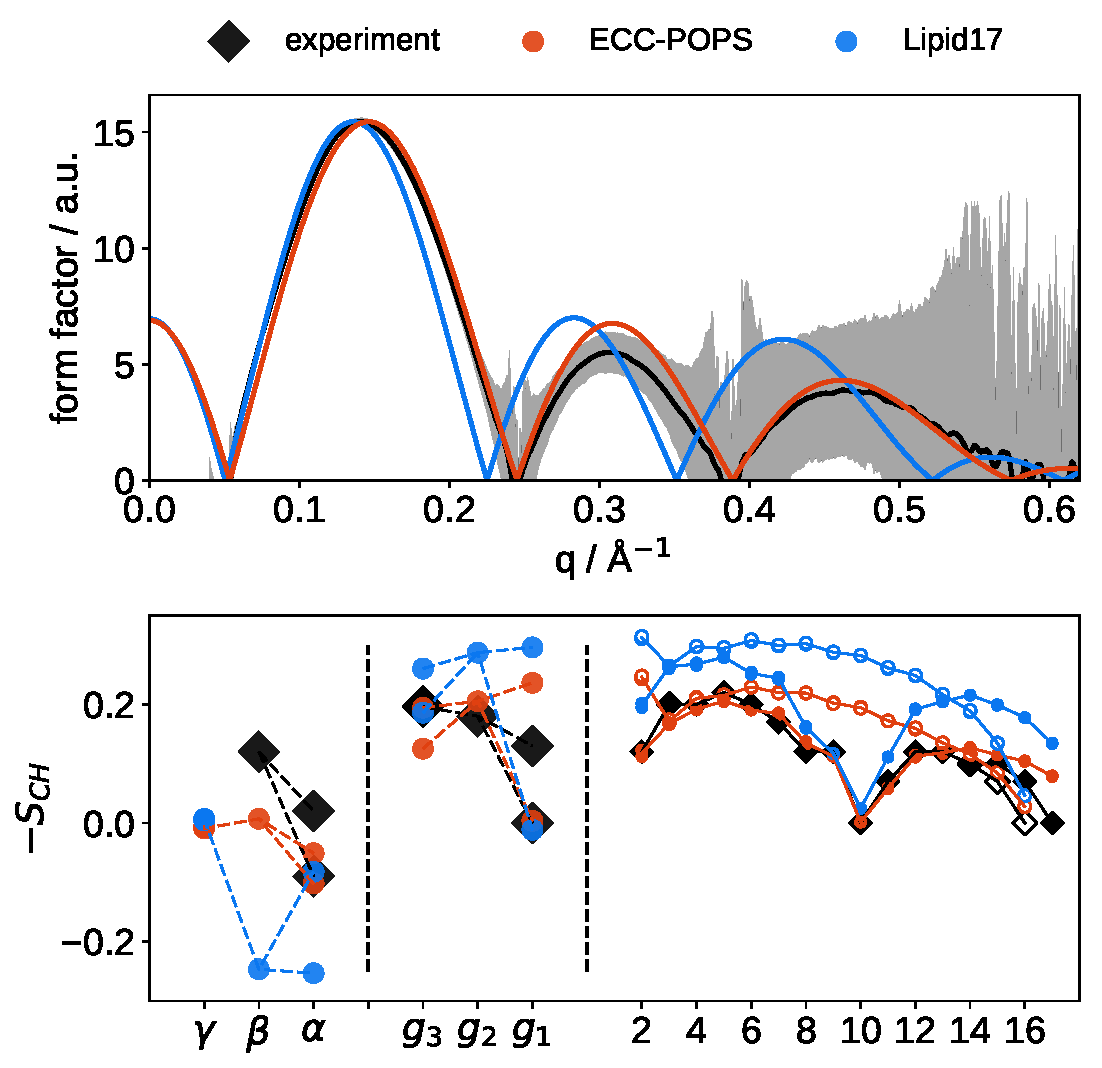
\includegraphics[width=\figwidth]{../img/ecc_pops/Order-parameters_form-factors_exp-L17-ECC-lipids.pdf}
  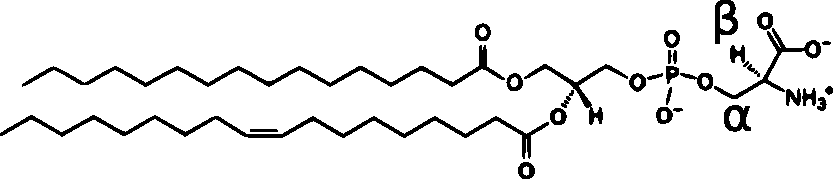
\includegraphics[width=\figwidth]{../img/ecc_pops/pops_chemfig.pdf} 
\hfill
  \caption{\label{simVSexpNOions_POPS} 
    \textbf{Top:} X-ray scattering form factors from simulations with Lipid17/Dang \citep{lipid17-future, dang2006} and 
    the ECC-POPS/ECC-ions \cite{martinek17, Pluhackova2016} compared with experiments~\citep{kucerka14} at 298~K. 
    \textbf{Middle:} Order parameters of POPS head group, glycerol backbone and acyl chains  
    from simulations with the Lipid17 \citep{lipid17-future} and the ECC-POPS models 
    compared with experiments at 298~K. \citep{nmrlipids_proj4}
    Open/closed symbols are used for palmitoyl/oleoyl chains of POPS. 
    \textbf{Bottom:} The chemical structure of POPS and the labeling of the carbon segments. 
  }  
\todo{J: flip the chemical structure so that it agrees with the left-to-right reading of the plot.}
\end{figure} 
 


\begin{table}[tb!] 
\centering
  \caption{Values of the area per lipid (APL) of POPS bilayers 
	   at 298~K with only \ce{Na^+} counterions and no additional ions. 
           Standard deviations are given. \label{tab:apls} } 
  \begin{tabular}{l|c } 
    \multicolumn{2}{c}{POPS} \\
    model          & APL / Å$^2$    \\ 
    \hline 
    Lipid17/Dang              & 53.5$\pm$ 1.7   \\ 
    Lipid17/ff99              & 57.9$\pm$ 1.7   \\ 
    \hline 
    ECC-POPS/ECC-ions         & 59.8$\pm$ 1.8   \\ 
    \hline 
    experiment (SDP model) \citep{kucerka14} & 62.3  \\ 
    \hline 
  \end{tabular} 
\end{table} 
 
We compared X-ray scattering form factors and NMR order parameters of bilayers
in pure water without any ions (or only counter ions)
from simulations and experiments. 
The experimental X-ray scattering form factors 
of a bilayer are well reproduced by ECC-POPS, 
while for Lipid17/Dang they are in a slight disagreement
(see Fig.~\ref{simVSexpNOions_POPS}). 
The agreement of Lipid17 can be improved by using different parametes for ions \cite{aqvist90},
which, however, bring other kinds of artifacts with them 
(e.g., incorrect pairing of ions, condensation at larger salt concentrations \cite{kohagen16, chen07, nmrlipids_proj4}). 

%The area per lipid is often used as a relatively simple structural parameter reporting on the bilayer properties and the packing of lipids. 
In order to obtain the area per lipid from experiments, modeling is used on top of the scattering factors \citep{kucerka14}. 
In ocntrast, this property is easily extracted directly from simulations with flat phospholipid bilayers. 
We compare the values from experiments and simulations in Table~\ref{tab:apls}. 



\begin{figure}[tbp!] 
  \centering 
  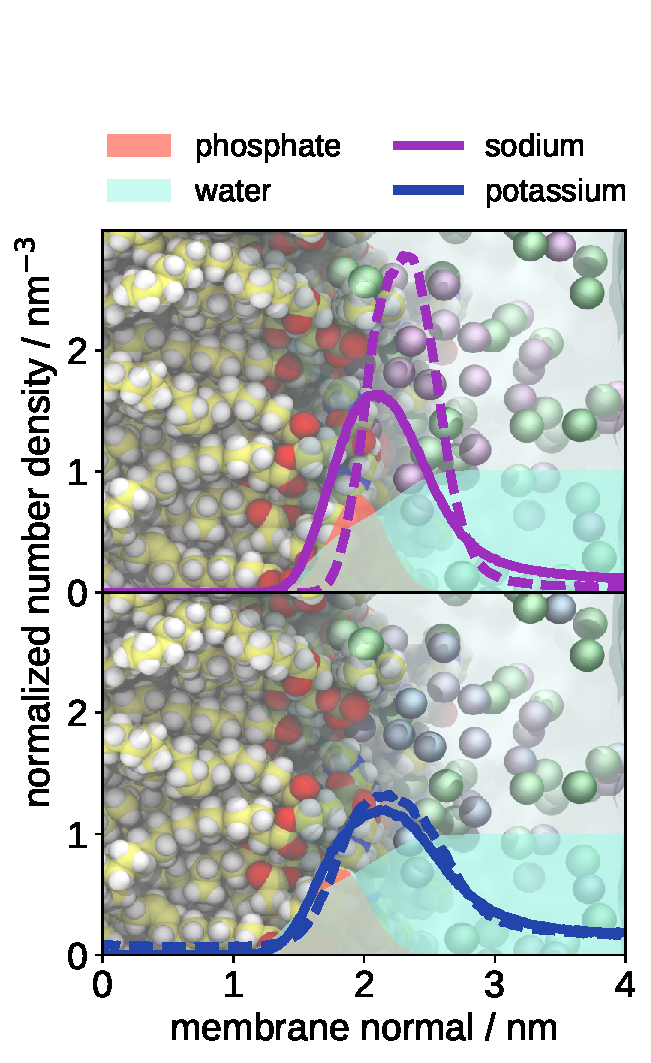
\includegraphics[height=\figheight]{../img/ecc_pops/density_profiles_na-k-counterions_wat_phos_compar_purePOPS_ecclipids-lipid17.pdf}
  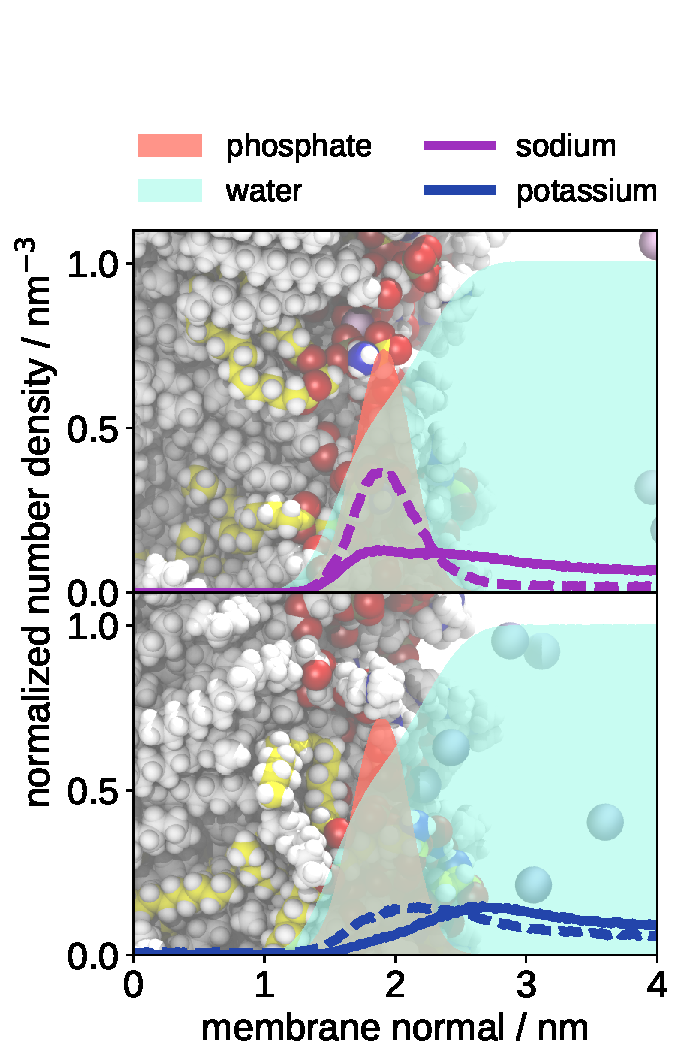
\includegraphics[height=\figheight]{../img/ecc_pops/density_profiles_na-k-counterions_wat_phos_compar_5PC-1PS_ecclipids-lipid17.pdf}
  \caption{\label{fig:POPS-counterions-dens}
    Number density profiles of \ce{K^{+}}, \ce{Na^{+}} counterions along the membrane normal axis 
    for the negatively charged bilayers composed of only POPS (left) or POPC:POPS (5:1, right) 
    using ECC-lipids/ECC-ions (solid lines) and Lipid17/Dang ions (dashed lines).  
    The density profiles of phosphate groups and water are divided by 4 and 100, respectively.  
}
\todo{JOE: add labels with the relative surface excess $\Gamma$, which are promised to be present in the text.}
\todo{JOE: split this figure into two: separate for POPS (to SI) and PC:PS 5:1 (main text)?}
\end{figure} 


While the agreement between the scattering form factors 
from the simulation of a pure POPS bilayer and experiment 
are excellent (Fig.~\ref{simVSexpNOions_POPS}),
there is a non-negligible difference between the values of the area per lipid in Table~\ref{tab:apls}. 
Since both values are derived from the scattering form factors through modeling of the electron density of the bilayer,
we cannot decide, which of the values is more reliable. 
In general, we can conclude that ECC-lipids
%the presented lipid models with ECC-lipids 
reproduce the experimental structural parameters of the lipid bilayers 
with a comparable accuracy to existing state-of-the-art lipid models~\citep{botan15, ollila16, Pluhackova2016}. 


\begin{figure}[tb!] 
  \centering 
  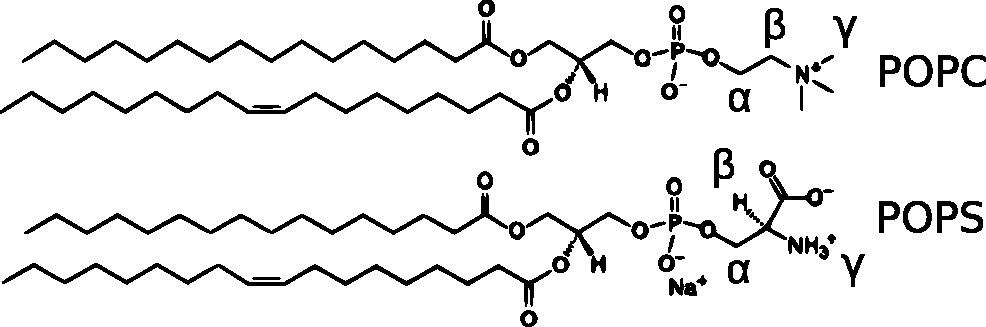
\includegraphics[width=\figwidth]{../Fig/lipids_chemfig_POPC_POPS.pdf} 
  \caption{ \label{fig:chemstruct_pc_ps} 
            The chemical structure of POPC and POPS 
            including the labeling of the carbon segments
            used in the measurements of order parameteres. 
  }  
\end{figure} 
 
The head group and acyl chain order parameters within ECC-lipids
are in general in a good agreement with the experimental values 
as shown in Fig. \ref{simVSexpNOions_POPS}. 
The acyl chain order parameters in particular agree with the experimental data within error bars.
The order parameters of the head groups are at an accuracy comparable to 
other currently available classical models of lipids \citep{botan15, catte16, Pluhackova2016, nmrlipids_proj4}. 
In particular, ECC-POPS is closer to the experimental order parameters 
than Lipid17 with either Dang \cite{smith94,chang1999,dang2006} 
or ff99 ions \citet{aqvist90}. 

%The head group order parameters $\alpha$ and $\beta$ are highly relevant for this work,
%as they are being used in the electrometer concept \cite{altenbach84, catte16, melcr18}.
%For POPC in pure water, the order parameter $\beta$ agrees well with the experiment, while the order parameter $\alpha$ is somewhat lower. 
The head group order parameters of PS are a bit more complicated 
compared to PC as the order parameter $\alpha$ exhibits a notable forking 
(i.e., the hydrogen atoms in the group give rise to different order parameters, see Fig.~\ref{simVSexpNOions_POPS}).
One of the order parameters of ECC-POPS, $\alpha_1$, agrees well with the experiment, 
while the other, $\alpha_2$, adopts a higher value underestimating the experimentally reported forking. 
There is only one order parameter $\beta$ in POPS, 
which has a higher value closer to zero in the ECC-lipids model than in experiment. 
Such a feature suggests that the model likely overestimates the orientational freedom of the PS head group. 

 
 
 
\subsection{Binding of counterions to negatively charged PC:PS bilayers and interactions between PC and PS head groups}

According to the electrometer concept,
the head group order parameters $\alpha$ and $\beta$ of PC lipids
change proportionally to the amount of bound charge
in a fixed ratio. \cite{seelig87,scherer87,roux90} 
This was demonstrated for a bound positive charge in simulations with POPC and 
cationic surfactants or aquaeous cations employing the ECC-POPC model \cite{melcr18}.
In this work, we will use the electrometer concept also for a bound negative charge 
using PS lipids as negatively charged surfactants. \cite{roux90} 

Unlinke in pure PC bilayers,
Interpreting the changes of the head group order parameters of 
mixed PC:PS lipid bilayers 
from both simulations and experiments
is complicated by the presence of counterions. \cite{nmrlipids_proj4}
In order to see the effects of different counterions, 
we performed simulations with \ce{Na+} and also with \ce{K+} counterions, 
which bind more weakly to phospholipids. \cite{nmrlipids_proj4, melcr18}
This can also be seen in the density plots of the counterions in Fig.~\ref{fig:POPS-counterions-dens},
which show a significantly reduced concentration of \ce{K+} ions 
at the membrane head group region compared to \ce{Na+}
for both PS and mixed PC:PS (5:1) bilayers. 

The slopes of the response of the PC head group order parameters $\alpha$ and $\beta$ 
in the mixed PC:PS (5:1) bilayer with \ce{K+} counterions
(Fig.~\ref{fig:delta_ordPar_NaCl_PC-PS_mix})
agree qualitatively well with experiments for both employed models,
i.e., for both Lipid14/17 and ECC-lipids. 
The same property from the simualtions with \ce{Na+} counterions, 
which were used in the experimental measurement,
are not as good, however.
In particular,
ECC-lipids have a weaker response of their PC head group order parameters compared to the experiments, 
while the simulations with Lipid17 model reveal a completely opposite trend.
This effect likely arises from an overestimated binding of the sodium cations to the phospholipids \cite{nmrlipids_proj4},
which is likely still present in a small amount also in the simulations with ECC-lipids. 
The large difference between the affinities of the employed lipid models to the counterions 
is visible in the density plots in Fig~\ref{fig:POPS-counterions-dens}. 

The order parameters of the PS head groups including their changes with the content of PC lipids
are challenging to capture correctly in classical MD simulation models. \cite{nmrlipids_proj4}
From such a perspective,
the changes of the PS head group order parameters from ECC-lipids 
with \ce{Na+}, and also \ce{K+}, counterions 
agree comparably well to the experimental measurements
(Fig.~\ref{fig:delta_ordPar_NaCl_PC-PS_mix}). 
Interestingly enough, 
although the Lipid17 model performed well with \ce{K+} counterions 
for the PC head group order parameter changes,
it does not agree in the equivalent changes in PS head groups
pointing at non-negligible effects of even relatively weakly binding cations 
on the structure of negatively charged lipids. 

Despite the great improvements in the overall structure of ECC-POPS 
and its response to PC lipids and counterions,
there is still a large room for improving it
to agree with the experimental measurements. 







\begin{figure*}[!tbp] 
  \centering 
  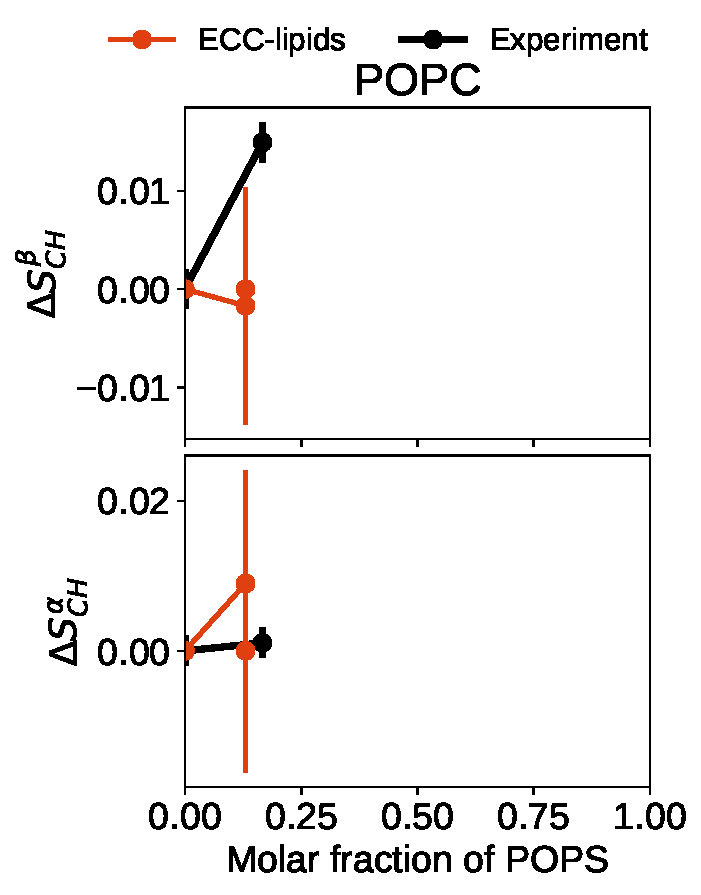
\includegraphics[height=\figheightsmall]{../Fig/order_parameters_changes_A-B_PC-PS_mix_POPC_nacl.pdf} 
  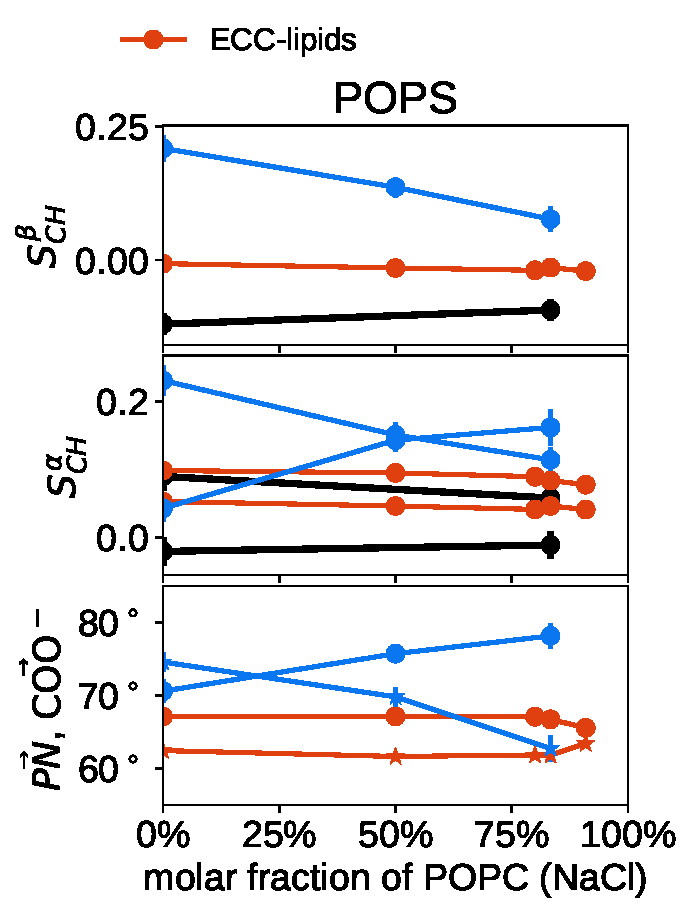
\includegraphics[height=\figheightsmall]{../Fig/order_parameters_changes_A-B_PC-PS_mix_POPS_nacl.pdf} 
  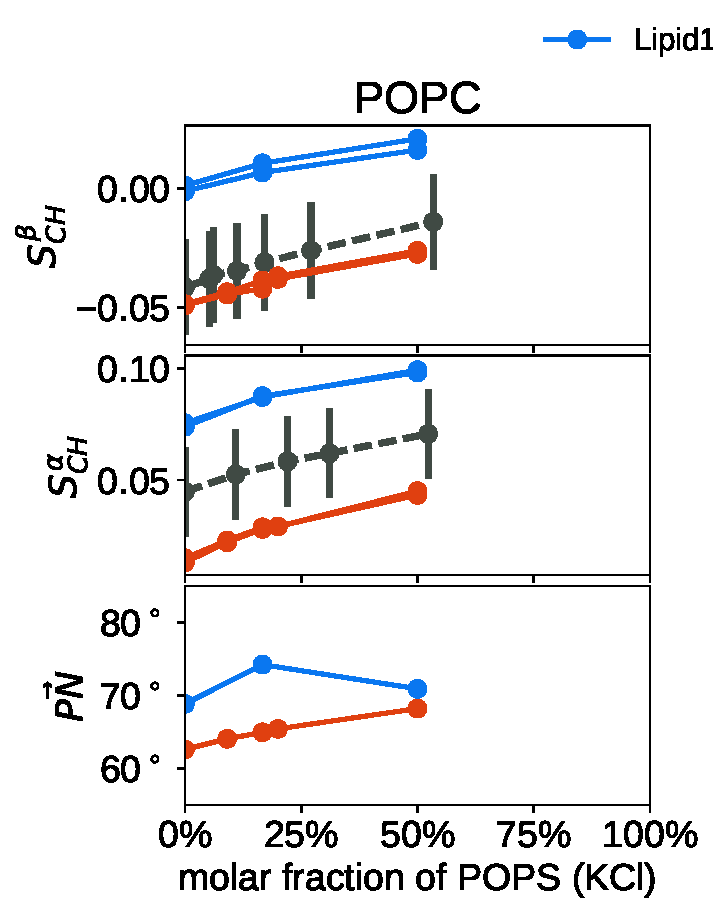
\includegraphics[height=\figheightsmall]{../Fig/order_parameters_changes_A-B_PC-PS_mix_POPC_kcl.pdf} 
  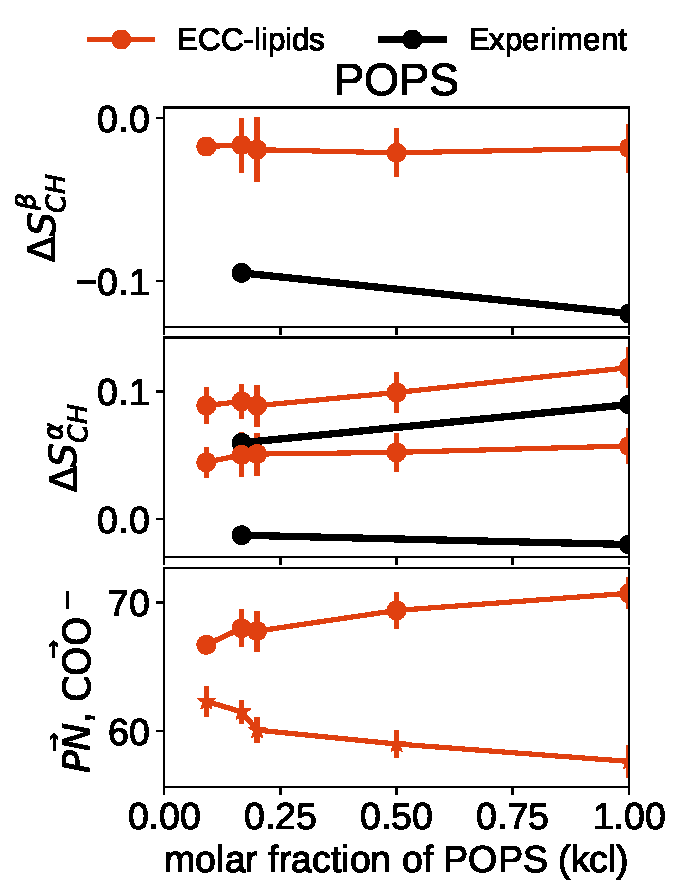
\includegraphics[height=\figheightsmall]{../Fig/order_parameters_changes_A-B_PC-PS_mix_POPS_kcl.pdf} 
  \caption{\label{fig:delta_ordPar_NaCl_PC-PS_mix} 
    The head group order parameters of a POPC:POPS (5:1) bilayer as a function of PS content
    with \ce{Na^+} (top) and \ce{K^+} (bottom) counterions from simulations with ECC-lipids and Lipid17 \cite{lipid17-future} 
    and experiments (only \ce{Na^+} counterions, but shown also in bottom plots). \cite{roux90}. 
    The underestimated response of ECC-lipids with \ce{Na^+} counterions 
    is likely due to a still slightly overestimated binding affinity of \ce{Na^+} to the phospholipids,
    which is corroborated by the series with \ce{K^+} counterions (lower affinity than \ce{Na^+}),
    where the response is closer to the experiment, which uses only \ce{Na^+} counterions. 
  }
\todo{JOE+SAMULI: split this figure into separate plots for PC and PS, 
and change the PS-plot x-axis to reflect the dilution of POPS by PC (now shows the content of PS). 
The experimental lines in the bottom plot shall be different to make clear that they are not with K counterions (gray dashed?).}
\end{figure*} 




 
 
 


\subsection{Molecular interaction and binding affinities of K$^+$ and Na$^+$ cations to mixed POPC:POPS (5:1) membrane} 
\label{sec:K_Na_added} 
 
 
\begin{figure}[tbp!] 
  \centering 
  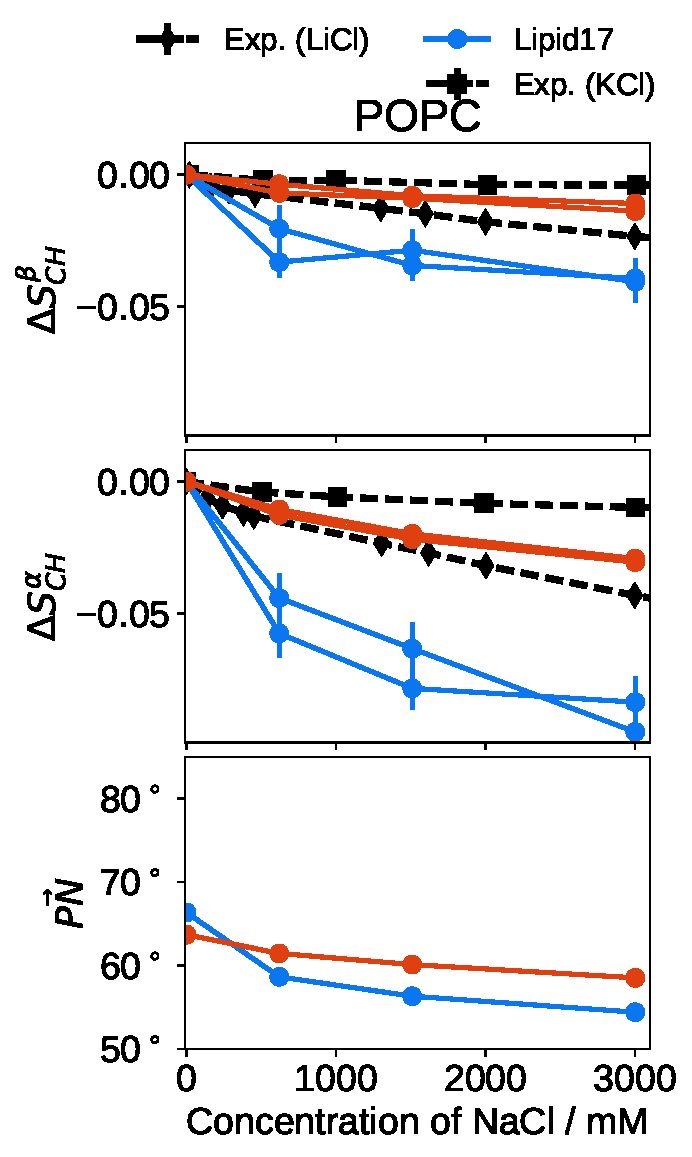
\includegraphics[height=\figheight]{../img/ecc_pops/order_parameters_changes_ecc-lip_L14_A-B-PN-COO_POPC_nacl.pdf} 
  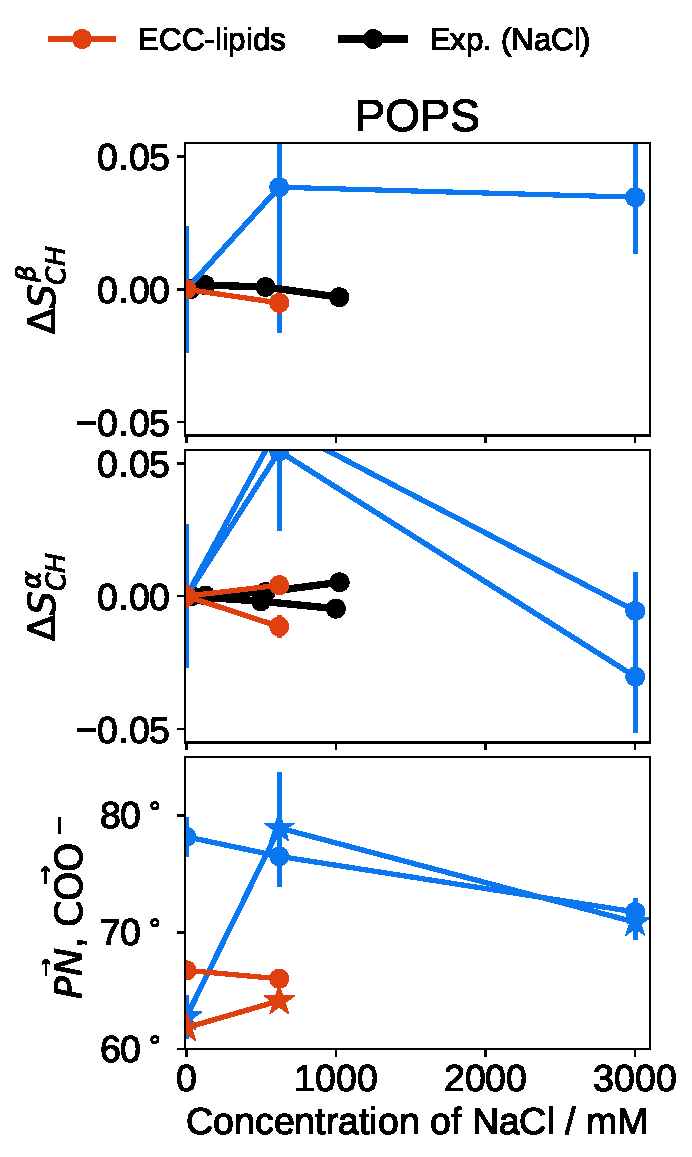
\includegraphics[height=\figheight]{../img/ecc_pops/order_parameters_changes_ecc-lip_L14_A-B-PN-COO_POPS_nacl.pdf} 
  \caption{\label{fig:delta_ordPar_NaCl_PCPS} 
    Changes of the head group order parameters $\alpha$, $\beta$ and the orientations of the carboxylate group and the P-N vector  
    of POPC (left) and POPS (right) phospholipids in a POPC:POPS 5:1 bilayer 
    as a function of \ce{NaCl} concentration in the buffer 
    from simulations with different force fields and experiments at 298 K. \citep{roux90}
    Because data with \ce{NaCl} are not available for POPC, 
    we show experimental data for \ce{LiCl} (dashed line, left) 
    as an upper bound for the magnitude of the response to \ce{NaCl}, 
    which has a lower affinity to phospholipid bilayers compared to \ce{LiCl} \citep{roux90}. 
    The orientation of the \ce{COO^-} group is defined as 
    the connector from the $\beta$ carbon to the carbon in \ce{COO^-} (stars, bottom right). 
  }
  \todo{SAMULI: Use the same y-axis scale in the bottom figures showing angles for POPC and POPS to ease the comparison.}
  \end{figure} 


\begin{figure}[tbp!] 
  \centering 
  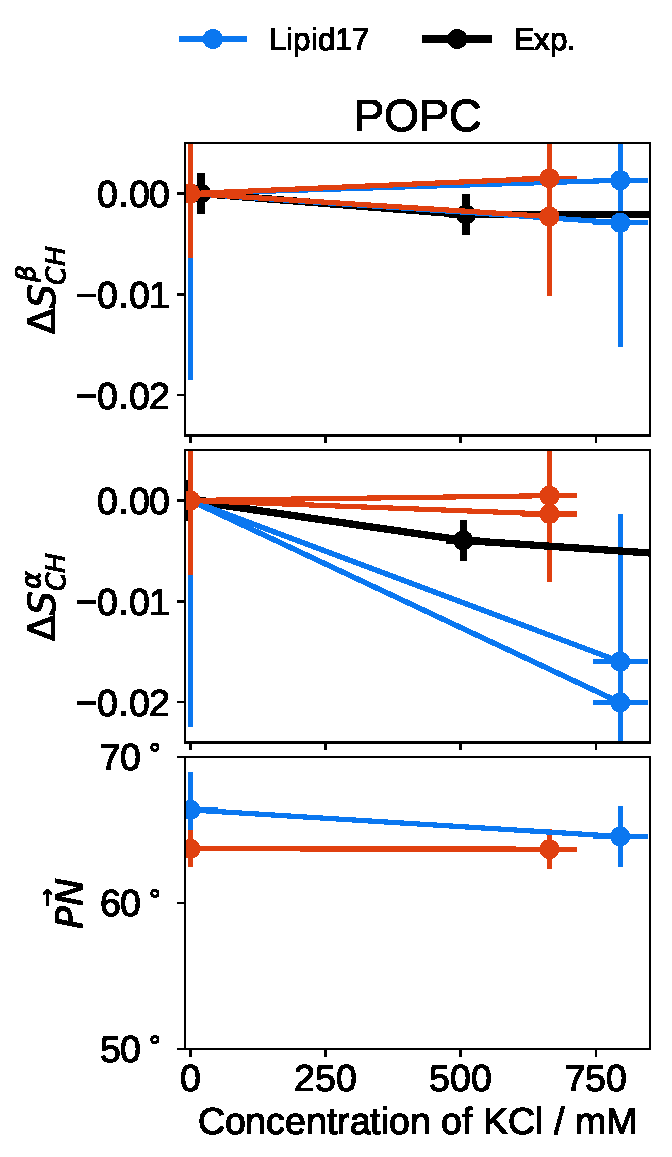
\includegraphics[height=\figheight]{../img/ecc_pops/order_parameters_changes_ecc-lip_L14_A-B-PN-COO_POPC_kcl.pdf} 
  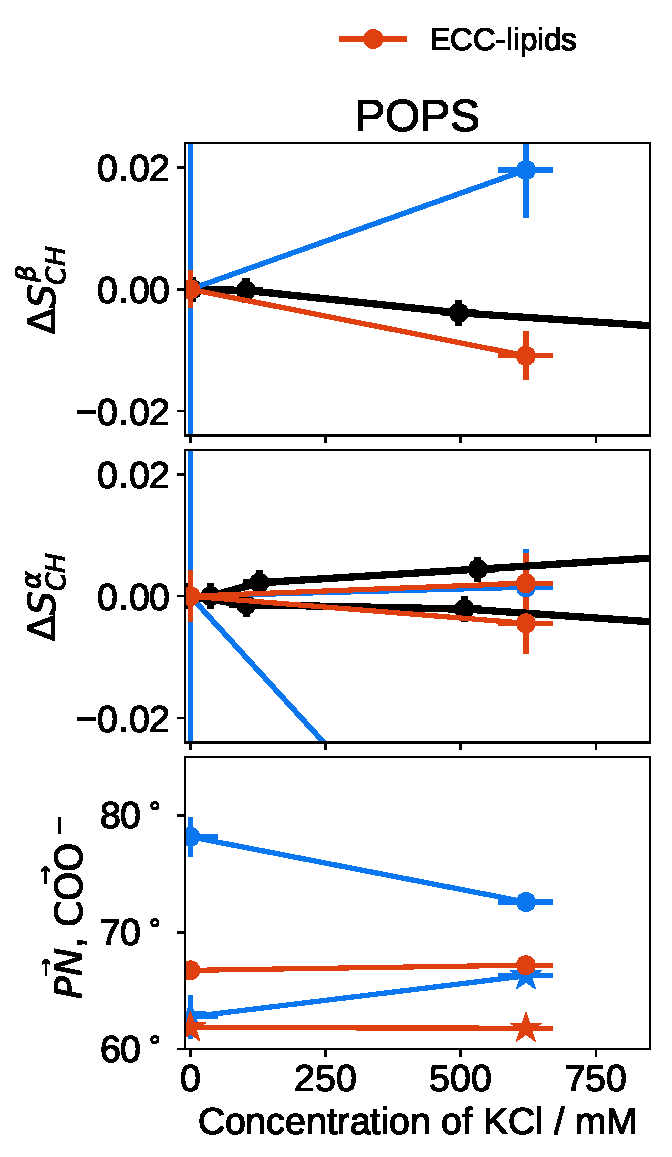
\includegraphics[height=\figheight]{../img/ecc_pops/order_parameters_changes_ecc-lip_L14_A-B-PN-COO_POPS_kcl.pdf} 
  \caption{\label{fig:delta_ordPar_KCl_PCPS} 
    Changes of the head group order parameters $\alpha$, $\beta$ and the orientations of the carboxylate group and the P-N vector  
    of POPC (left) and POPS (right) phospholipids in a POPC:POPS 5:1 bilayer 
    as a function of \ce{KCl} concentration in the buffer 
    from simulations with different force fields and experiments at 298 K. \citep{roux90}
    The orientation of the \ce{COO^-} group is defined as 
    the connector from the $\beta$ carbon to the carbon in \ce{COO^-} (stars, bottom right). 
  }
  \todo{SAMULI: Use the same y-axis scale in the bottom figures showing angles for POPC and POPS to ease the comparison.}
\end{figure} 
 

% This§: 
% NA/K binding status, 
% how we tried finding a model (NMRlipids4), and 
% how it was futile
% 
The binding of \ce{Na^+} cations to phospholipid bilayers 
is not generally agreed on between simulations 
\citep{bockmann03,sachs04,berkowitz06,cordomi09}
and experiments 
\citep{cevc90,tocanne90,hauser76,herbette84,uhrikova08}.
We attempted to find a model, 
which would successfully interpret the experiments on binding of \ce{Na^+}
to neutral and negatively charged phospholipid bilayers \citep{akutsu81, roux90} 
in our works \citep{catte16, nmrlipids_proj4}.
After testing the currently available force fields for phospholipids,
we concluded
that the interactions are generally overestimated in magnitude in almost all models 
but Lipid14 (PC) \citep{dickson14}, resp. Lipid17 (PS) \citep{lipid17-future}. 
This model yields a semi-quantitative agreement with the experimentally measured small changes of the order parameters \cite{catte16}
when used with the model of ions by \citet{aqvist90}. 
However, when used with a more accurate model of ions by \citet{Pluharova2014, martinek17},
the model overestimates the binding affinity of \ce{Na^+}
measured with lipid electrometer concept. \citep{melcr18}
In total, these results suggest that improvements 
in the lipid parameters are required for more accurate interactions even with monovalent cations. 
\citep{catte16, melcr18, nmrlipids_proj4}


% This§: 
% we have developed a model that can describe the NMR exp. using ECC
% 
Generally improved behaviour 
of the POPC and POPS head group order parameters 
with \ce{NaCl} or \ce{KCl} concentrations 
was achieved through the combination of models 
ECC-lipids and ECC-ions \citep{martinek17, kohagen16, Pluharova2014}. 
Simulations with these models 
reveal a good agreement with the NMR experiments 
for both neutral and negatively charged membranes.
The results are plotted for \ce{NaCl} in Fig. \ref{fig:delta_ordPar_NaCl_PCPS}, 
and for \ce{KCl} in Fig. \ref{fig:delta_ordPar_KCl_PCPS}. 


% This§: 
% Other models do not yield good reponse, but
% ECC-lipid describe the changes well
% => Elect. polar. necessarry.
% 
The interaction with \ce{K^+}, which binds very weakly to both neutral and negatively charged membranes, 
renders a qualitatively different response of the order parameter $S^\beta$ in POPS 
in the mixed negatively charged bilayers compared to the neutral bilayers. 
While the order parameter $S^\beta$ increases for both \ce{Na^+} and \ce{Ca^{2+}},
it decreases in the presence of \ce{K^+}
(\ce{KCl}:  Fig.~\ref{fig:delta_ordPar_KCl_PCPS}, 
 \ce{NaCl}: Fig.~\ref{fig:delta_ordPar_NaCl_PCPS}, and
\ce{CaCl2}: Fig.~\ref{fig:delta_ordPar_CaCl_PCPS}). 
Despite the tremendous effort in the development of classical MD models of lipids, however,
there is no such model, 
which would agree with the experimental trends for these salt solutions \cite{nmrlipids_proj4}. 
In contrast, ECC-lipids with ECC-ions capture the different response 
of the order parameters $S^{\beta}$, $S^{\alpha _1}$ and $S^{\alpha _2}$ in POPS 
to various concentrations of \ce{NaCl} and \ce{KCl} in a good agreement with the experiments
(\ce{KCl}:  Fig.~\ref{fig:delta_ordPar_KCl_PCPS}, 
 \ce{NaCl}: Fig.~\ref{fig:delta_ordPar_NaCl_PCPS}). 
Such a dramatic improvement in the structural parameters 
demonstrates that including electronic polarization in phospholipids is crucial 
even for interactions with soft cations like \ce{K^+}. 



\begin{figure}[tbp!] 
  \centering 
  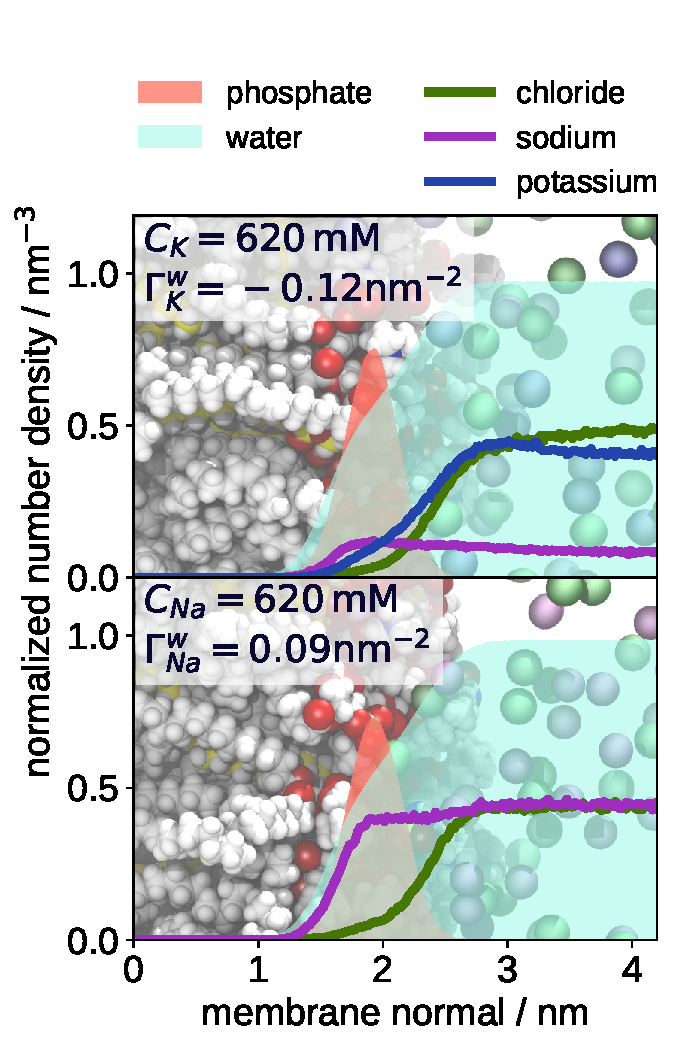
\includegraphics[width=\figwidth]{../img/ecc_pops/density_profiles_na_k_cl_wat_phos_models-compar_5-6_NaCl-and-KCl-series.pdf}
  \caption{\label{fig:nacl-dens_PCPS} 
    Number density profiles of \ce{K^{+}}, \ce{Na^{+}} and \ce{Cl^-} along the membrane normal axis 
    for the negatively charged membranes with the composition of 5\,PC:1\,PS using ECC-lipids and ECC-ions
    from simulations with added concentrations of \ce{KCl} or \ce{NaCl}.  
    The top    profile shows the simulation with an additional \ce{KCl} concentration and \ce{Na^+} counterions. 
    The bottom profile shows the simulation with an additional \ce{NaCl} concentration and \ce{Na^+} counterions, which are not distinguished from the added salt. 
    The density profiles of phosphate groups and water are divided by 4 and 100, respectively.  
  }
\end{figure} 


% This§: 
% adsorption and affinities of Na and K to PC:PS memb
% from densities and rel.surf.excess
% 
%in  Fig.~\ref{fig:POPS-counterions-dens} (only counterions)
%and Fig.~\ref{fig:nacl-dens_PCPS}        (additional salt concentrations), 
%
The affinities of \ce{Na^+} and \ce{K^+} to phospholipid membranes
can be described by their relative surface excesses with respect to water, $\Gamma ^{w} _{ion}$. 
Such a quantity compares the adsorption of ions to the adsorption of water molecules at an interface 
without the necessity of defining a Gibbs dividing surface. \citep{melcr18, chattorajBOOK}
Interestingly enough, \ce{K^+} maintains negative values of $\Gamma^{w}_{K}$ even for the negatively charged PC:PS~(5:1) bilayer.
This is also evident from the density plots in  Fig.~\ref{fig:nacl-dens_PCPS}
showing that the density profile of \ce{K^+} along the membrane normal 
decays clearly faster towards the membrane centre compared to the density of water. 
In contrast, the density profile of \ce{Na^+} has a shoulder 
at the region of the phosphate groups,
which demonstrates that sodium cations adsorb weakly to the membrane interface compared to the aquaeous solution
by yielding a small positive value of $\Gamma^{w}_{Na}$.

\todo{JOE: Add a discussion about the still slightly overestimated affinity of \ce{Na^+}.}





 
 


\subsection{Molecular interaction and binding affinities of \ce{Ca^{2+}} cations to mixed POPC:POPS (5:1) membrane} 
\label{section:lip-ion_ca}

\begin{figure}[tbp!] 
  \centering 
  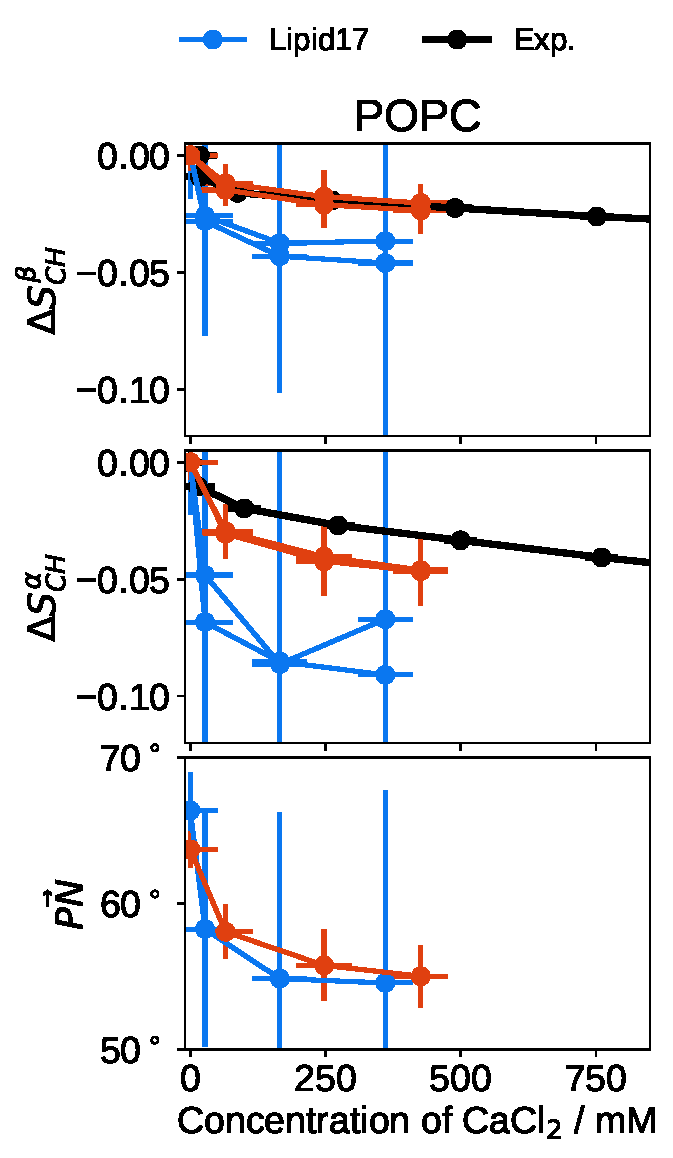
\includegraphics[height=\figheight]{../img/ecc_pops/order_parameters_changes_ecc-lip_L14_A-B-PN-COO_POPC_cacl.pdf} 
  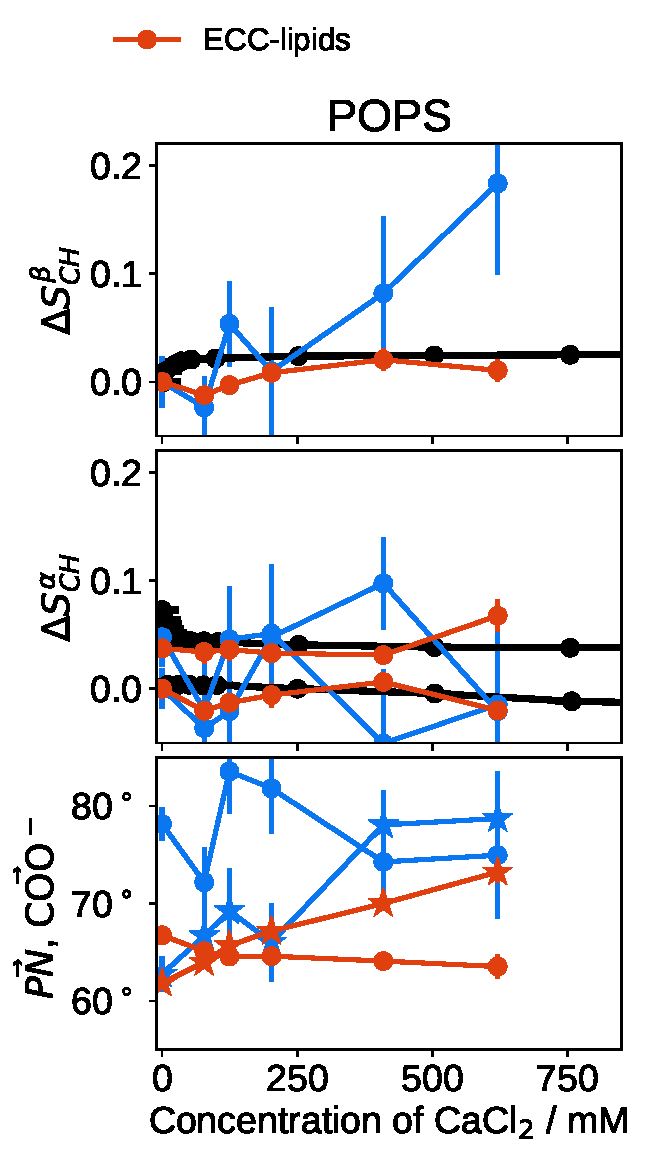
\includegraphics[height=\figheight]{../img/ecc_pops/order_parameters_changes_ecc-lip_L14_A-B-PN-COO_POPS_cacl.pdf} 
  \caption{\label{fig:delta_ordPar_CaCl_PCPS} 
    Changes of the head group order parameters $\alpha$, $\beta$ and the orientations of the carboxylate group and the P-N vector  
    of POPC (left) and POPS (right) phospholipids in a POPC:POPS 5:1 bilayer as a function of \ce{CaCl2} concentration 
    in bulk ($C_{ion}$) from simulations with different force fields and experiments at 298~K. \citep{roux90}
    The orientation of the \ce{COO^-} group is defined as 
    the connector from the $\beta$ carbon to the carbon in \ce{COO^-} (stars, bottom right).
  }
  \todo{SAMULI: Use the same y-axis scale in the bottom figures showing angles for POPC and POPS to ease the comparison.}
\end{figure} 



The interaction of various cations including calcium 
with  neutral and also negatively charged lipid bilayers
was thoroughly compared between simulations and experiments 
from the point of the electrometer concept \cite{roux90, seelig87, altenbach84}
in the references~\citenum{catte16, nmrlipids_proj4}. 
It was concluded that the interaction of calcium with zwitterionic PC bilayers 
is generally overestimated in all studied models \cite{catte16},
while none of the models was capable of interpreting the NMR structural parameters
with the negatively charged PC:PS (5:1) bilayers \cite{nmrlipids_proj4}. 
Accounting for the electronic polarization was identified as 
a non-negligible correction to the interaction between cations and POPC bilayers in Ref.~\cite{melcr18}. 
Here, we demonstrate that the same approach 
significantly improves the description of calcium binding 
also to the negatively charged PC:PS (5:1) bilayers. 
In correspondence with the Ref.~\citenum{nmrlipids_proj4},
we also use the changes of the head group order parameters $S^\alpha$ and $S^\beta$ 
in PC and PS lipids 
to quantify the binding affinity of the calcium cations
and the induced structural changes
(Fig.~\ref{fig:delta_ordPar_CaCl_PCPS}). 
To directly connect to the previous works \citep{catte16, nmrlipids_proj4}
and to mark the improvement after treating electronic polarizability, 
we show simulation results from ECC-lipids and also from Lipid17 \citep{lipid17-future}. 
While the response of the order parameters of PC to \ce{CaCl2} concentrations
is qualitatively correct in the Lipid14/17 model \cite{lipid17},
it is quantitatively comparable to the experimental trends in ECC-lipids. 
Moreover, the structure of PS head group is fundamentaly improved
after accounting for the electronic polarization 
(Fig.~\ref{fig:delta_ordPar_CaCl_PCPS}). 


Increasing concentrations of \ce{CaCl2} 
induce a systematic decrease of the order parameters $S^\alpha$ and $S^\beta$ 
in both neutral POPC bilayers \cite{catte16, melcr18}
as well as in the negatively charged PC:PS (5:1) bilayers \cite{nmrlipids_proj4, roux90}. 
The change of the head group order parameters 
are well reproduced only by ECC-lipids in Fig.~\ref{fig:delta_ordPar_CaCl_PCPS}. 


The structural changes in POPS induced by increasing concentrations of \ce{CaCl2} 
are very challenging to interpret from both experiments \cite{roux90} 
and also from MD simulations \cite{nmrlipids_proj4}. 
The changes of the order parameters $S^\alpha$ and $S^\beta$ in PS head groups from simulations 
are not found to follow the experimental profiles, 
nor any common trend,
with the currently available models \cite{nmrlipids_proj4}. 
In Fig.~\ref{fig:delta_ordPar_CaCl_PCPS},
we plot these structural parameters for one of the models in that work, Lipid17, 
and for ECC-lipids. 
Although the agreement between ECC-lipids and experiments is far from optimal,
the general trends and behaviour even at highly concentrated solutions of \ce{CaCl2} 
are well captured by the model. 
For example the order parameter $\beta$ in POPS 
adopts a saturated value in experiments and ECC-lipids,
but it is growing with the \ce{CaCl2} concentration in Lipid17.
In addition, 
the forking of the order parameters $\alpha$ 
is almost constant in the experiment and ECC-lipids,
but it varies greatly in th Lipid17. 


The changes of the order parameters $\alpha$ and $\beta$ at low \ce{CaCl2} concentrations
have a steep onset at low concentrations in the negatively charged bilayers compared to neutral POPC bilayers. 
However, such a detail is not captured by ECC-lipids
indicating the necessity for further improvements.
The source of this discrepancy may arise 
from the interactions between PC and PS lipids and with \ce{Na^+} counterions,
from the sub-optimal structure of the lipids (Fig.~\ref{simVSexpNOions_POPS},
and also possibly from the approximate mean-field treatment of the electronic polarization. 


It has been pointed out in previous experimental works
that the conformational flexibility of PS head groups 
is different from other lipids \cite{browning80}. 
While the static shielding tensor of PS is not substantially different from PC or PE, 
the $^{31}$P~$T_1$ relaxation times are significantly shorter for PS. 
It is suggested that the PS head group is more rigid compared to the other phospholipids, 
which is also corroborated by a larger chemical shielding anisotropy of PS \cite{browning80}. 

We have investigated this effect using the mean orientations of P-N and \ce{COO^-} vectors 
(defined and plotted in Fig.~\ref{fig:delta_ordPar_CaCl_PCPS}). 
While the mean angle between the P-N vector of PC head group and the membrane normal
decreased by 11$^\circ$ from 64$^\circ$ to 55$^\circ$
 at 620~mM buffer concentration of \ce{CaCl2},
the mean orientation of the P-N vector in the PS head group has 
decreased only by 3$^\circ$ from 67$^\circ$ to 64$^\circ$ 
in the same concentration range. 

Such a largely diminished flexibility 
may arise from the binding of calcium to the \ce{COO^-} group in PS. 
Whe have measured the mean orientation of the \ce{COO^-} group 
as the connector of the carbon atoms 
forming the bond between the group and the $\beta$-carbon of the phospholipid. 
The mean angle between the \ce{COO^-} vector and the membrane normal
changes by $11^\circ$ from $62^\circ$ to $73^\circ$ (more towards the membrane interior)
 at 620~mM buffer concentration of \ce{CaCl2}.
The conformational flexibility of the PS head group is hence restrained 
by the binding of calcium cations to the \ce{COO^-} group, 
which reorients towards the membrane interior and to the phosphate region, 
where calcium cations bind predominantly. 



\begin{figure}[htbp!] 
  \centering 
  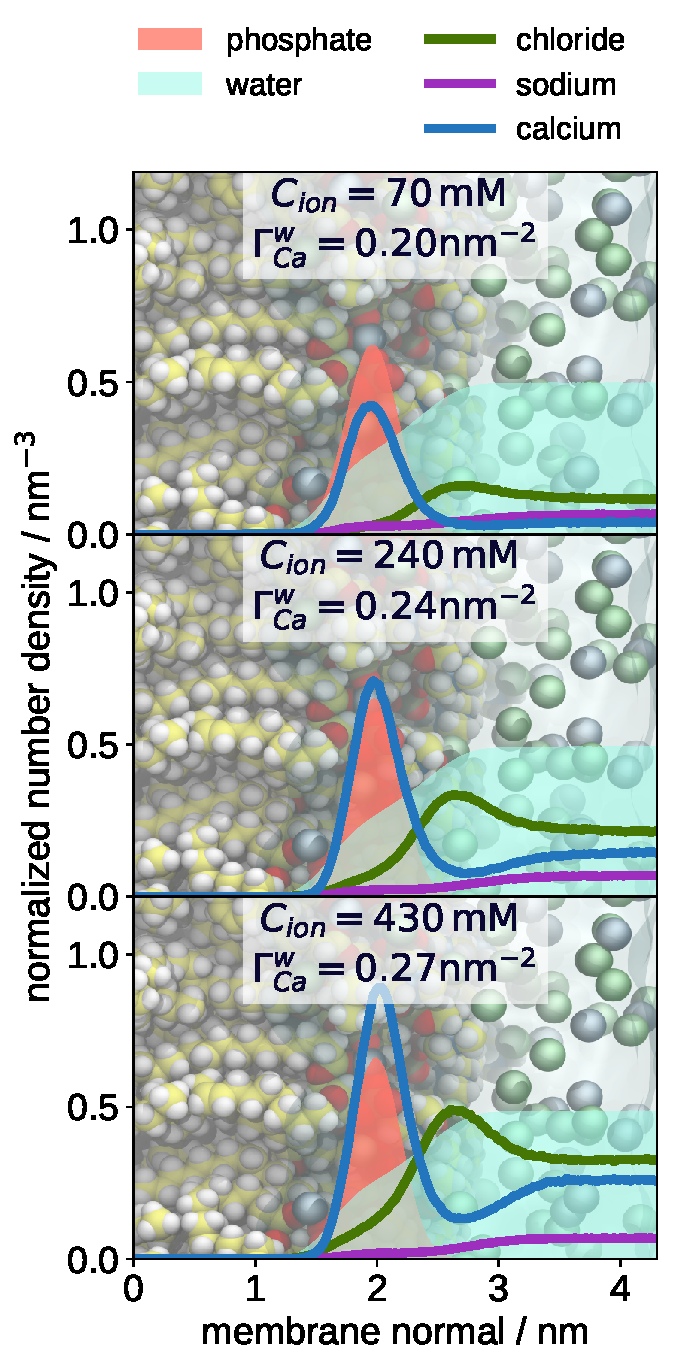
\includegraphics[width=\figwidth]{../img/ecc_pops/density_profiles_ca_na_cl_wat_phos_models-compar_1-3_CaCl2-series.pdf}
  \caption{\label{fig:cacl-dens_PCPS} 
    Number density profiles of \ce{Ca^{2+}}, \ce{Na^{+}} and \ce{Cl^-} along the normal of the membrane starting at the centre
    for the negatively charged membrane with the composition 5\,PC:1\,PS
    at various bulk concentrations of \ce{CaCl2} from simulations with ECC-lipids. 
    All profiles contain \ce{Na^+} counterions and an additional concentration of \ce{CaCl2}. 
    In order to visualize the density profiles with a scale comparable to the profile of \ce{Ca^{2+}},  
    the density profiles of~\ce{Cl^-} ions are divided by 2, and 
    the density profiles of phosphate groups and water are divided by 5 and 200, respectively.  
  }
  \todo{SAMULI: We should compare to the density profiles from Lipid17 simulations. These are also needed for NMRlipids IV.}
\end{figure} 
 

The binding of calcium cations to the phospholipid bilayer is shown 
in the density profiles of \ce{Ca^{2+}}, \ce{Na^+} counterions 
and also \ce{Cl^-} ions in Fig.~\ref{fig:cacl-dens_PCPS}. 
Clearly, after accounting for the electronic polarizability, 
the population of the cations in the phosphate region is significantly diminished. 
\todo{JOE: The density plot still needs to be changed to show both Lipid17 and ECC-lipids, and to support this argument.}
Still, the dominant contribution to the binding of calcium comes from the phosphate groups. 
Interestingly enough,
although the \ce{COO^-} groups increase the affinity of calcium towards PS compared to PC,
 there is no extra density at the outmost surface of the membrane. 
This can be understood from the point of the structural rearangements of the \ce{COO^-} group, 
which take place during the interactions with calcium cations
described above and in Fig.~\ref{fig:delta_ordPar_CaCl_PCPS}. 


The higher affinity of calcium to PS head groups compared to PC
is well demonstrated using the relative surface excess, $\Gamma ^w _{Ca}$,
summarized in Table~\ref{tab:binding}. 
While $\Gamma^{w}_{Ca}$ at a neutral POPC bilayer
is       $\Gamma^{w}_{Ca} = 0.06\mathrm{nm^{-2}}$, 
its value for the PC:PS (5:1) bilayer is $\Gamma^{w}_{Ca} = 0.24\mathrm{nm^{-2}}$
at comparable buffer concentrations  $350 \, \mathrm{mM}$ resp. $400\, \mathrm{mM}$. 



\begin{table}[tb!] 
\centering
  \caption{Bulk concentrations, $C _{Ca}$, and buffer concentrations, $C' _{Ca}$, of Ca$^{2+}$;
           relative surface excess of calcium with respect to water ($\Gamma_{Ca}^{\rm water}$); 
           and percentages of the population 
           of bound Ca$^{2+}$ to various moieties 
           in a neutral membrane composed of POPC
           and in a negatively charged membrane with the composition 5\,PC:1\,PS.
           \label{tab:binding}} 
  \begin{tabular}{ l | c c } 
	                     &  5\,POPC:1\,POPS &  POPC   \\
	\hline
	$C _{Ca}\,/\,\mathrm{mM}$  &  $240\pm 10 $  &  $280\pm 10 $  \\
	$C'_{Ca}\,/\,\mathrm{mM}$  &  $400\pm 10 $  &  $350\pm 10 $  \\
	$\Gamma_{Ca}^{\rm water}\, / \,\mathrm{nm}^{-2}$  &  $0.24 \pm 0.01 $  &  $0.06 \pm 0.01 $  \\
	\hline
                             &  \multicolumn{2}{c}{ } \\
        interacting moiety   &  \multicolumn{2}{c}{percentage of bound \ce{Ca^{2+}} } \\
	\hline
	     PC              &   59   &  100   \\
	     PO$_4$    in PC &   41   &   67   \\
	     carbonyls in PC &   <1   &   ~1   \\
	\hline
	     PS              &    8   &        \\ 
	     PO$_4$  in PS   &    2   &        \\
	     COO$^-$ in PS   &    4   &        \\
	     carbonyls in PS &   <1   &        \\
	\hline
	both PC and PS       &   33   &        \\
  \end{tabular} 
\end{table} 




% Description of no. conctacts counting
Further details about the interactions of \ce{Ca^{2+}} with various moieties in POPC or POPS
were obtained by counting contacts between the cations and the oxygen atoms of the lipids
similarly as was done in \cite{melcr18}. 
The threshold for counting a contact was set to $0.3\,\mathrm{nm}$, 
which encompasses the first peak of the radial distribution function between the cations and the oxygen atoms of the lipids. 


% Populations from contacts
The percentages of the populations of membrane-bound calcium cations for various membrane moieties 
are summarized in Table~\ref{tab:binding}.
Even though the negatively charged membrane contains only 18\% of POPS, 
approximately 41\% of the total population of bound calcium cations is in contact with PS lipids
with 8\% bound only to them. 
This corroborates the intrinsically higher affinity of PS lipids to calcium cations compared to neutral PC lipids. 
% Where Calcium interacts
POPC interacts with the calcium cations almost entirely through its phosphate group 
in both neutral \cite{melcr18} and negatively charged membranes. 
Interactions of \ce{Ca^{2+}} with carbonyl groups are also present, 
however, they are always accompanied by interactions with phosphate groups. 
%but a very small negligable amount much below 1\%. 


Relative probabilities of \ce{Ca^{2+}} complexes with a certain number of lipids are presented in Fig.~\ref{fig:cacl_complexes}. 
Calcium cations that are bound only to PC in the mixed bilayer with PS 
behave similarly as in the pure PC bilayer
maintaining comparable probabilities for clustering one, two, or even three PC lipids together. 
In contrast, PS lipids prefer 1:1 ratio with \ce{Ca^{2+}},
which may also be due to their low molar fraction in the the mixed bilayer. 
In total, however, the negatively charged membrane has its stoichiometry 
shifted towards complexes with three phospholipids and one calcium. 
This is obviously due to the presence of POPS, 
which also contributes to the pre-formed one- and two-membered clusters of POPC. 
Clusters of four or more lipids were not observed in either membrane. 

%This is also reflected in the increased probability 
%of a single phospholipid interacting with two \ce{Ca^{2+}} cations 
%compared to the neutral POPC bilayer, 
%where such a probability is almost negligable. 
% Not shown through numbers, however, I have the plots to back it. 

Timescales associated with the binding of calcium cations from solution to the membrane
are plotted for each binding event as a histogram in Fig.~\ref{fig:hist_residence_times}. 
Using these plots, we can estimate that 90\% of the residence times of any calcium cation 
will be lower than $60\,\mathrm{ns}$ for pure POPC neutral bilayer 
and shorter than $200\,\mathrm{ns}$ for the mixed 5\,PC:1\,PS negatively charged bilayer. 
The longest observed residence times in the simulations were $141\,\mathrm{ns}$ for the neutral membrane 
and $485\,\mathrm{ns}$ for the negatively charged membrane. 
Both estimates of the residence times come from simulations with comparable concentrations of around $250\mathrm{mM}$;
the simulation with the neutral membrane has a bulk concentration of calcium $C_{ion} = 280\mathrm{mM}$, 
whereas the simulation with the negatively charged membrane has a bulk concentration of calcium $C_{ion} = 240\mathrm{mM}$. 

In summary, the results from ECC-lipids suggest 
that the exchange of calcium between the POPC bilayer and the solvent 
occurs at the order of $\sim$10--100~ns, 
which is significantly faster than observed in simulations 
with other presently available non-polarizable models of lipids and ions~\citep{javanainen17, catte16}. 
Our results suggest 
that simulation trajectories with a characteristic length of several hundreds of nanoseconds 
are necessary to capture the binding of calcium to neutral POPC bilayers 
in equilibrium when more realistic \emph{polarizable} force fields are used. 
Interestingly enough, almost an order of magnitude longer simulations
are required for the negatively charged bilayers. 

 
%In addition to such estimates of the time scales, we used the Markov model on top of the simulation with the negatviely charged mixed bilayer
%to calculate the time of the mean first passage of calcium from solution to the membrane (and in reverse) resulting in $55\,\mathrm{ns}$  ($165\,\mathrm{ns}$). 

%\todo{Fluxes: committor analysis, dominant fluxes (table and figure)}
%From the spectrum of the transition matrix, we also observe that 
%the slowest transitions are associated with the binding to two or three phosphate moieties from either PC or PS,
%which are also among the states with the highest probabilities.
%The net fluxes of calcium cations from solution to such states also form a large contribution to the total flux ($\approx 45\%$). 
%\todo{Make a table and a figure of the state probabilities and fluxes to support this statement.}. 
%Analysis of the possible binding pathways of calcium cations to the negatively charged mixed bilayer 
%reveal that the cations mostly enter the membrane bound states directly from solution 
%without complicated transitions at the time scales of the order of the lag time of the Markov state model, $25\,\mathrm{ns}$. 


FOLLOWING: lit. search on recent literature, which shall be discussed in this work. 


\todo{EDIT: Taken from NMRlipids4 as an interesting information, to be edited.}
The dehydrated complexes of PS headgroup and calcium ions can also lead to the
phase separation \cite{hauser77,kurland79,hauser85,feigenson86,mattai89,roux90,roux91}.
%
CHARMM36 force field \cite{klauda10,venable13} combined with 2D infrared spectroscopy
suggests that calcium ions interacts only with the carboxylate group of PS lipids \cite{valentine18}, while
the same force field without the NBfix parameters together with the NMR chemical shifts and
REDOR experiments suggests a significant binding affinity also to the phosphate region \cite{hallock18}.
On the other hand, simulations with the Berger force field \cite{berger97,mukhopadhyay04}
combined with fluorescent and vibrational sum frequency spectroscopy suggested a significant
calcium binding also to the carbonyls in the acyl chains \cite{melcrova16}. 


% Details of interactions between calcium and phospholipids (PC and PS) .
% Major conclusions correct, only the model (Berger) over-exaggerates certain features. 
From abstract of \cite{melcrova16}://
Namely, time-resolved fluorescent spectroscopy of lipid vesicles 
and vibrational sum frequency spectroscopy of lipid
monolayers are used to characterize local binding sites of calcium in zwitterionic and anionic model
lipid assemblies, while dynamic light scattering and zeta potential measurements are employed for
macroscopic characterization of lipid vesicles in calcium-containing environments. To gain additional
atomic-level information, the experiments are complemented by molecular simulations that utilize an
accurate force field for calcium ions with scaled charges effectively accounting for electronic polarization
effects. We demonstrate that lipid membranes have substantial calcium-binding capacity, with several
types of binding sites present. Significantly, the binding mode depends on calcium concentration with
important implications for calcium buffering, synaptic plasticity, and protein-membrane association. 

And From conclustions of \cite{melcrova16}://
Calcium ion binding sites are heterogeneous both from the point of view of binding affinity and their positioning
in the membrane. The character of the calcium binding varies with calcium concentration; this issue is of par-
ticular importance as significant concentration spikes of calcium ions occur along calcium signaling pathways.
The present results support the conjecture that lipid membranes, in particular the negatively charged inner leaflet
of the plasma membrane, can act as effective calcium buffers upon calcium ions entering the cytosol. Of equal
importance is the fact that the strong binding of this ion significantly alters the membranes by means of reduction
of their hydration, lipid mobility, and lateral inter-lipid distance. Such local conformational membrane remod-
eling may play a significant role in modulation of lipid-protein interactions as well as membrane-membrane
interactions. Overall, the phenomena related to calcium ions-membrane interactions demonstrated here point to
their diverse roles in biological systems.


% Ca2+ induces much slower dynamics of lipids when PS is present,
% this does not happen with PC
From Ref.~\cite{valentine18}://
To summarize, calcium binding to PS lipids slows the dynamics at the ester position and introduces more heterogeneous molecular environments. 
The slowdown cannot be attributed to complete ester dehydration or decreased hydrogen bonding to water, so we interpret these results as evidence that the lipid headgroups adopt more rigid but disordered conformations on the molecular level. 
The decrease in dynamics observed experimentally indicates that the network of hydrogen bonds between lipids and water at the polar-nonpolar interface becomes slower, as it was shown by Karathanou and Bondar (34). 
This is bolstered by recent NMR work showing that binding to Ca2+ induces two different rigid conformations in the glycerol backbone of lipid headgroups (18).
We have investigated the molecular origin of the rigidification and decreased lateral diffusion, finding that calcium binding does not dehydrate the ester region, but even with only 10\% PS lipids, the local dynamics slow around the esters. The slower local dynamics provide a molecular explanation for the Ca2+-dependent decreases in fluidity observed on longer length and timescales.
There is considerable room for further improvement in the force fields for ion-membrane interactions. Particularly, small differences in short-range interactions may determine the local geometries (34
). Most of our conclusions are, however, based on long-range effects (i.e., electric field generated by the ion at significant distances from the carbonyl groups), which are less sensitive to the details of the force field. 




% 2 major head group configurations of PS in 30-70 PC-PS mix -- paper 1
From Ref.~\cite{boettcher11}://
 In this study, combining magic angle spinning (MAS) solid-state NMR (SSNMR) measurements of isotopically labeled serine headgroups in mixed lipid bilayers with molecular dynamics (MD) simulations of PS lipid bilayers in the presence of different counterions, we provide site-resolved insights into the effects of Ca2+ on the structure and dynamics of lipid bilayers. Ca2+-induced conformational changes of PS in mixed bilayers are observed in both liposomes and Nanodiscs, a nanoscale membrane mimetic of bilayer patches. Site-resolved multidimensional correlation SSNMR spectra of bilayers containing 13C,15N-labeled PS demonstrate that Ca2+ ions promote two major PS headgroup conformations, which are well resolved in two-dimensional 13C-13C, 15N-13C, and 31P-13C spectra. The results of MD simulations performed on PS lipid bilayers in the presence or absence of Ca2+ provide an atomic view of the conformational effects underlying the observed spectra.
but the NMR ...
 Spectra were acquired of 70\% POPS* and 30\% POPC Nanodiscs with 2 mM Ca2+ using an MAS rate of 10 kHz on a 600 MHz (1H frequency) spectrometer
and but the MD sim was done only for pure POPS bilayer and no other counterions but Ca2+ with CaCl2 concentration.

% 2 major head group configurations of PS in 30-70 PC-PS mix -- paper 2
% extended analysis and insight. 
From Ref.~\cite{hallock18}://
(conclusions) We investigated the atomistic details of how membranes containing anionic PS lipids are shaped into their functional state by Ca2+ ions. The lipid phosphate groups and the captured ions are made readily accessible to interact with proteins. Using extensive MD simulations with a lipid-accelerated membrane representation, we demonstrated that PS lipid nanoclusters are formed by two distinct PS headgroup conformations that are induced by Ca2+ ions, which bind to the lipids in a specific manner. Importantly, detailed characterization of MD-derived lipid nanoclusters and geometries of individual PS lipids agree with SSNMR measurements on two different spatial scales. (1) The chemical shifts show the accuracy of capturing the chemical environment around a single lipid in either of the two long-lived conformations, and (2) the Ca2+-coordinated PS lipid tetramer is a basic structural unit that is involved in membrane sculpturing. By studying the effects of ions on membranes containing anionic lipids, we have characterized a baseline behavior and structures of the lipids. These results will be important in interpreting the role of lipids in future protein–membrane studies, and they demonstrate that MD HMMM simulations combined and validated by SSNMR methodologies are effective at capturing high-resolution signature lipid structures that are stabilized by membrane-active agents in complex membrane environments.
but ... again, the experiment with nanodiscs (and also the bilayer simulation with HMMM) 
uses 70:30 PS:PC ratio, which induces PS clustering.
 -> hence the markable difference between their figure 3 and our figure \ref{fig:cacl_complexes}
 - they observe most probable Ca2+ clusters of 2, then 3, 1 and 4 PS together
 - while we see rather only 1PS per ca2+ in Figure \ref{fig:cacl_complexes}
On the other hand, I see correspondence with the observed longer life time ( stronger interaction?)
with \ce{COO-} group in PS in \cite{hallock18} in Fig 4, for both Ca2+ and Na+. 
This is followed by PO4 in both cases. 
In the case of Ca2+, the ratio of the observed life time is also in line with our findings, that 
the interaction with the PO4  and COO- together is of a smaller abundance compared to the interactions of the individual groups themselves, yet comparable to that of PO4. 
Their Figure 5 shows the distributions of O-Ca-Cb-N dihedral angle
revealing separate populations of the PS head groups. 
These two structures are also compared in therm of P-Cg distances, 
which can be measured from NMR REDOR exp. 
It is concluded that since the two distinct populations in P-Cg distance can be represented with the 
dihedral distributions, 
they also likely represent the distinct populations. 
 -> plotting the distribution of O-Ca-Cb-N dihedral angle may be also a good idea for us (SI?)
     -> NMRlipids 4 in SI \cite{nmrlipids_proj4} plots this information: 
           - C36 agress with the distribution in \cite{hallock18}
           - Lipid17 (and Slipids) are almost identical to C36
           - but the structure of the COO- is highly different (dih angle Ca-Cb-Cg-Og)






\begin{figure}[tb!] 
  \centering 
  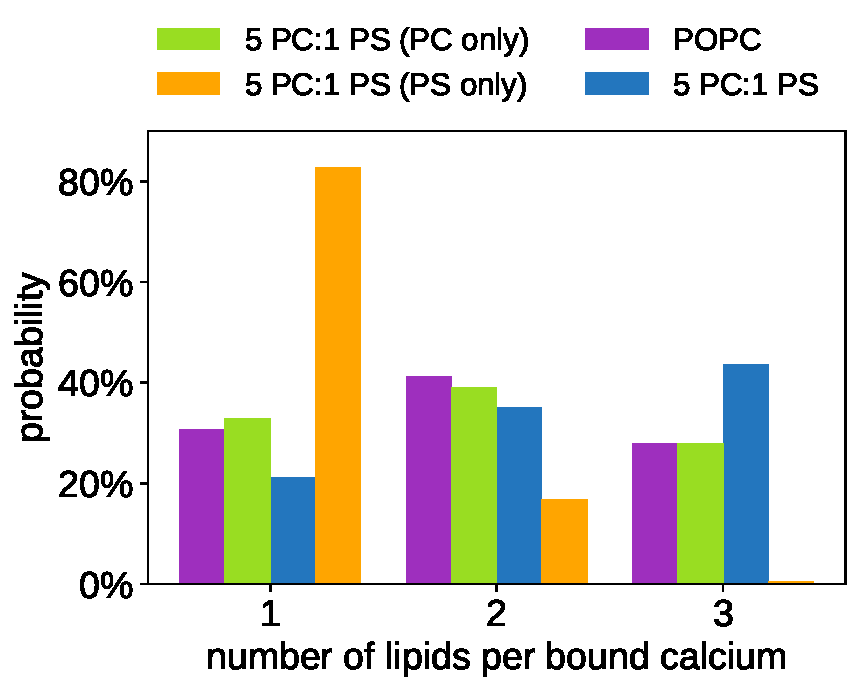
\includegraphics[width=\figwidth]{../img/stoichiometry_CaCl2_comparison_Ecc-lipids_PC-vs-PCPS.pdf} \\ 
  \caption{\label{fig:cacl_complexes} 
      Relative probabilities of existence of \ce{Ca^{2+}} complexes 
      with a certain number of lipids.  
      All lipids were taken into account with the exception of the complexes in light green and orange, 
      for which we counted only contacts with POPC resp POPS from the mixed 5\,PC:1\,PS negatively charged bilayer. 
      The calculated probabilities of the calcium-lipid complexes also reflect only POPC (light green) resp POPS (orange). 
      Probabilities were taken from simulations with comparable bulk concentrations of calcium around 250~mM. 
      Clusters of four or more lipids were not observed in either membrane. 
      Simulation data for POPC bilayers were taken directly from \cite{melcr18}. 
  } 
\end{figure} 











 
 
 





%\todo{Stationary distribution: Make a figure documenting the populations of bound \ce{Ca^{2+}} cations (like I have in the presentation) that would accompany Table \ref{tab:Ca_binding_PCPS}. 
%This will roughly correspond to the PC stoichiometry plot \ref{fig:cacl_complexes}. }




\begin{figure}[tb!]
  \centering
  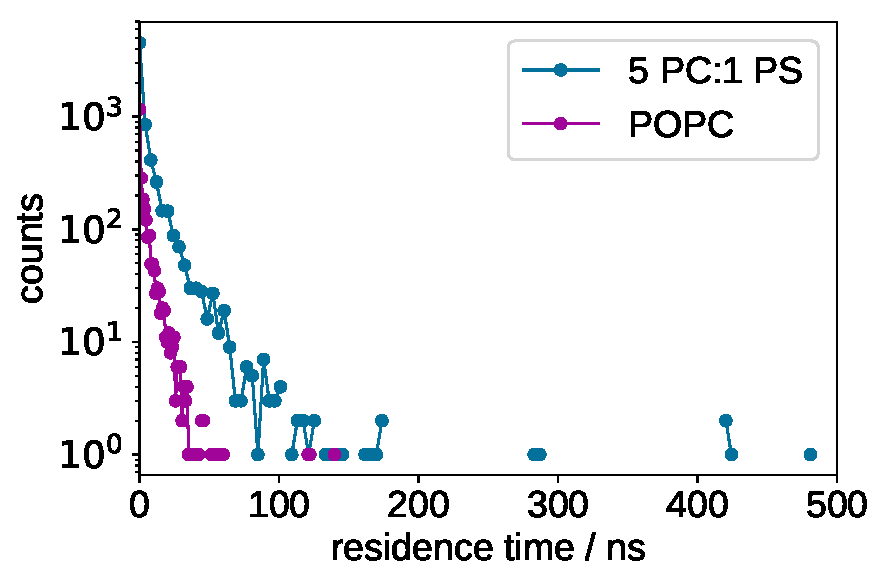
\includegraphics[width=\figwidth]{../img/histogram_bound_times_26CaCl2_comparison_PC-PCPS.pdf}
  \caption{\label{fig:hist_residence_times}
   Histograms of residence times of \ce{Ca^{2+}} 
   in a neutral membrane composed of POPC (orange)
   and in a negatively charged membrane with the composition 5\,PC:1\,PS (blue)
   from simulations with ECC-lipids and ECC-ions.
   The simulation with the neutral membrane has a bulk concentration of calcium $C_{ion} = 280\mathrm{mM}$, 
   the simulation with the negatively charged membrane has a bulk concentration of calcium $C_{ion} = 240\mathrm{mM}$. 
   In the simulation with the neutral membrane, 
   90\% of the residence times of calcium cations are
   shorter than $60\,\mathrm{ns}$, % exactly $53\,\mathrm{ns}$                                                                          
   with the longest observed residence time being $141\,\mathrm{ns}$. 
   In the simulation with the negatively charged membrane, 
   90\% of the residence times of calcium cations are
   shorter than $200\,\mathrm{ns}$, % exactly $53\,\mathrm{ns}$                                                                          
   with the longest observed residence time being $485\,\mathrm{ns}$. 
   Simulation data for POPC bilayers were taken directly from \cite{melcr18}. 
   }
\end{figure}





 
 



 
 
 
 
 
\section{Conclusions} 

\todo{SAMULI: I have putted here two preliminary sentences}
Applying ECC to POPS lipids improves cation binding affinity to membranes
mixed with POPC and also the response of PS headgroup to the bound cations.
However, further improvement of the parameters is needed to fully reproduce the
details of calcium binding to PS headgroups.
 
\listoftodos
 

% If you have acknowledgments, this puts in the proper section head. 
\begin{acknowledgement} 
% Put your acknowledgments here. 
P.J. acknowledges support from the Czech Science Foundation (grant no. 16-01074S)  
and from the Academy of Finland via the FiDiPro award. 
Computational resources were supplied by the Ministry of Education, Youth and Sports 
of the Czech Republic under the Projects CESNET (Project No. LM2015042) and CERIT-Scientific 
Cloud (Project No. LM2015085) provided within the program Projects of Large Research, 
Development and Innovations Infrastructures. 
O.H.S.O. acknowledges financial support from 
Integrated Structural Biology Research Infrastructure of 
Helsinki Institute of Life Science (Instruct-HiLIFE). 
\end{acknowledgement} 
 
\begin{suppinfo} 
 
%A listing of the contents of each file supplied as Supporting Information 
%should be included. For instructions on what should be included in the 
%Supporting Information as well as how to prepare this material for 
%publications, refer to the journal's Instructions for Authors. 
 
%The following files are available free of charge. 
%\begin{itemize} 
%  \item Filename: brief description 
%\end{itemize} 
 
\end{suppinfo} 
 
 
\bibliography{refs.bib} 
 
\end{document} 
 

